%% =============================================================================
%% IST submission — Overleaf package (flat layout)
%%
%% Build on Overleaf (pdfLaTeX + BibTeX, default settings):
%%   pdflatex main
%%   bibtex main
%%   pdflatex main && pdflatex main
%%
%% Files (paths relative to main.tex):
%%   main.tex
%%   cap3_article_body.tex
%%   cover_letter.tex
%%   results/qa_assessment_summary.tex
%%   results/kappa/kappa_report.tex
%%   results/auxiliary/aux_qa_summary.tex
%%   results/auxiliary/aux_ft_summary.tex
%%   results/auxiliary/aux_reft_summary.tex
%%   results/auxiliary/kappa/aux_kappa_report.tex
%%   results/ec5_recovery/ec5_recovery_report.tex
%%   results/sensitivity/sensitivity_report.tex
%%   results/final_review/missing_references.bib
%%   results/segress_checklist.tex
%%   results/human_validation/human_kappa_report.tex
%%   results/human_validation/human_confusion_report.tex
%% =============================================================================

\documentclass[review,3p,times]{elsarticle}

%% --- Math + tables ---
\usepackage{amsmath,amssymb}
\usepackage{booktabs}
\usepackage{multirow}
\usepackage{array}
\usepackage{tabularx}
\usepackage{makecell}
\usepackage{longtable}
\usepackage{caption}

%% --- Figures ---
\usepackage{graphicx}
\usepackage{tikz}
\usetikzlibrary{arrows.meta,positioning,shapes}
\usepackage{pgfplots}
\pgfplotsset{compat=1.18}

%% --- Misc ---
\usepackage{enumitem}
\usepackage{xcolor}
\usepackage{hyperref}
\hypersetup{colorlinks=true, linkcolor=blue!50!black, citecolor=blue!50!black, urlcolor=blue!50!black}
%% Allow DOI/URL strings to wrap inside table cells (pdflatex).
\usepackage{xurl}

%% --- Bibliography style: Elsevier numeric + sorted ---
\bibliographystyle{elsarticle-num}

%% --- Zenodo replication-package DOI (new deposit, 2026-08-14) ---
\newcommand{\zenododoi}{10.5281/zenodo.21939600}
\newcommand{\zenododoiurl}{https://doi.org/\zenododoi}

%% --- Round-2 placeholders: filled after `python -m pipeline.round2_validation --compute`.
%% Must not remain in the submitted PDF: `grep -n "\tbd" *.tex` must return nothing.
\newcommand{\tbd}[1]{\textcolor{red}{\textbf{[#1]}}}

\journal{Information and Software Technology}

\begin{document}

%% =========================
%% Front matter
%% =========================
\begin{frontmatter}

\title{Process Mining and Stochastic Modeling for Software Process
       Forecasting: A Systematic Mapping Study with an LLM-Assisted Protocol}

%% Authors
\author[pucpr]{Rodrigo Almeida de Oliveira\corref{cor1}\fnref{orcid1}}
\ead{rodrigo.almeida1@pucpr.edu.br}

\author[pucpr]{Juliano de Paulo Ribeiro\fnref{orcid2}}
\ead{juliano.ribeiro@pucpr.edu.br}

\author[pucpr]{Edson Emilio Scalabrin\fnref{orcid3}}
\ead{scalabrin@ppgia.pucpr.br}

\cortext[cor1]{Corresponding author.}

\fntext[orcid1]{ORCID: 0009-0009-6310-4126}
\fntext[orcid2]{ORCID: 0009-0004-3605-485X}
\fntext[orcid3]{ORCID: 0000-0002-3918-1799}

\affiliation[pucpr]{
  organization={Pontif\'icia Universidade Cat\'olica do Paran\'a (PUCPR), Graduate Program in Informatics (PPGIa)},
  city={Curitiba},
  state={PR},
  country={Brazil}
}

%% --- Abstract (150–300 words, structured) ---
\begin{abstract}
\textbf{Context.}
Software processes generate event data that process mining (PM) and
stochastic models can use for forecasting, yet their integration for
software development lifecycle (SDLC) prediction is reported only
anecdotally.
\textbf{Objective.}
To map the state of the art at the intersection of process mining,
stochastic modeling, and machine-learning forecasting applied to software
processes; to identify research gaps; and to propose a research agenda.
\textbf{Method.}
We report a systematic mapping study against
SEGRESS~\cite{kitchenham2023segress}. The mapping protocol was not
pre-registered. The human check of the screen was. Searches ran on
12~April~2026. An LLM screened 2{,}340 working-set and 3{,}807 auxiliary
records. The success bar, set before the judgements, was Recall $\geq 0.90$.
\textbf{Results.}
The LLM list has 340 studies. Two predate 1994 and are removed, leaving
338. Human Recall on the working-set sample is 0.630 (29 of 46; Wilson
95\% CI 0.486--0.755). Auxiliary Recall is 0.725 (235 of 324). After
de-duplication the corpus is 506 studies. Family-code findings use the
cuts named in each sentence, not the 506. One study in 429 matches
process mining, a stochastic model, and forecasting. F2 and F5 are
unconfirmed model counts.
\textbf{Conclusion.}
The family-code picture is descriptive and predictively thin. It is not a
census of the 506, because the screen missed eligible studies. PATHCAST is
future work, not a result of this mapping.
\textbf{Limitations.}
The second pass used the abstract for almost every record. Seventy-seven
added studies were read from the title alone.
\end{abstract}

\begin{keyword}
Systematic Mapping Study \sep
Process Mining \sep
Stochastic Modeling \sep
Software Process Forecasting \sep
LLM-Assisted Screening \sep
Mining Software Repositories
\end{keyword}

%% --- Highlights (3–5 bullets, ≤85 chars each) ---
\begin{highlights}
\item Human check of the LLM screen: Recall 0.630 and 0.725.
\item This revision maps 506 distinct studies after de-duplication.
\item Findings F1--F5 still describe the 338, except the triple count.
\item One of 429 coded studies joins mining, stochastic models, and forecasting.
\item Replication package: Zenodo DOI 10.5281/zenodo.21939600.
\end{highlights}

\end{frontmatter}

%% =========================
%% Body
%% =========================
\section{Introduction}
\label{sec:slr-intro}

Software organisations routinely need to answer forecasting questions about
their own development process: when a feature will be delivered, how long an
issue will remain open, or whether a release will slip. The data needed to
answer them already exists as a by-product of everyday work---commits, issue
transitions, pull requests, code reviews, and CI/CD executions are all
time-stamped events. Three research communities have developed techniques
that can exploit these traces, largely independently of one another.
\emph{Process mining} (PM) discovers, checks, and enhances process models
from event logs, and has been applied to software repositories since the
work of Cook and Wolf~\cite{cook1995,cook1998} and Rubin et
al.~\cite{rubin2007}. \emph{Stochastic modelling}---Markov chains,
stochastic Petri nets, Monte Carlo simulation---has a long tradition in
software reliability and process simulation~\cite{whittaker1994,ali2014simulation}.
\emph{Machine-learning-based prediction} dominates mining-software-repositories
research on defects, effort, and outcomes~\cite{kagdi2007msr,hall2012fault},
and, in the business-process domain, predictive process
monitoring~\cite{marquezchamorro2018predictive}. Combining them is attractive
because each covers a weakness of the others: PM provides an empirically
grounded process structure, stochastic models turn that structure into
probability distributions over future paths and durations, and ML can
correct systematic errors using context features. Whether, and how far, the
literature has actually combined them for software processes is not known.

\paragraph{Related secondary studies.} Existing secondary studies each cover
one side of this space. In business process management, predictive process
monitoring has been surveyed and benchmarked for outcome
prediction~\cite{teinemaa2019outcome}, remaining-time
prediction~\cite{verenich2019remaining}, and in
general~\cite{marquezchamorro2018predictive}, but on business event logs
rather than software development processes. General mappings of process
mining applications~\cite{garcia2019pmmapping,thiede2018pmorg} treat software
engineering as one domain among many and do not address forecasting. Within
software engineering, secondary studies have covered process simulation
modelling~\cite{zhang2010simulation,ali2014simulation}, process mining of
FLOSS event logs~\cite{mukala2015floss}, software process mining with Petri
nets~\cite{thamizharasan2016petri}, continuous software monitoring backed by
process mining~\cite{stepanov2026continuous}, repository
mining~\cite{kagdi2007msr}, and defect prediction~\cite{hall2012fault}. Four
of these (\cite{zhang2010simulation,mukala2015floss,thamizharasan2016petri,stepanov2026continuous})
fall within our scope and were retained as included studies under EC4
(Table~\ref{tab:criteria}), which excludes only secondary studies that do
\emph{not} address PM or stochastic methods in software engineering. None of
them maps the joint use of process mining, stochastic modelling, and
forecasting on software development data, and none reports how often the
three are combined. Establishing that baseline is the gap this mapping study
addresses.

\paragraph{Why the mapping matters.} For researchers, a structured map shows
which combinations have been tried, on which SDLC phases and data sources,
and with what evidence, so that integration work can build on what exists
instead of re-deriving it. For practitioners, it indicates which parts of a
process-aware forecasting toolchain are mature (discovery and conformance
checking on repository data) and which remain research problems. For the
methodology of secondary studies, the review is also a deployment of
LLM-assisted screening whose selection error we measure against a
pre-registered human reference standard, following
LLM4SCREENLIT~\cite{llm4screenlit2025}. The mapping protocol itself was
not pre-registered. The human check of the screen was pre-registered before
the round-2 judgements.

\paragraph{Study design and contributions.} We report a systematic mapping
study against SEGRESS~\cite{kitchenham2023segress}, following the mapping
guidelines of Petersen et al.~\cite{petersen2015}, the evidence-based software
engineering guidelines of Kitchenham and Charters~\cite{kitchenham2007}, and
the snowballing procedure of Wohlin~\cite{Wohlin2014}. The review addresses
three research questions, each decomposed into two sub-questions, covering
the application landscape of process mining in SDLC contexts, the techniques
and prediction methods employed, and the degree of integration between
process mining and stochastic forecasting. Its contributions are (i)~a
classification of the coded rows, on the cuts named in each sentence, by
SDLC phase, data source, and technique family; (ii)~family-code counts (F1, F3, F4) on the cuts
named in each sentence, which this revision did not re-mark, plus two
model counts (F2, F5) that a human re-read did not confirm; (iii)~the SPMF taxonomy and a four-direction research agenda; and (iv)~a
measured account of the LLM-assisted selection, including where it failed.
The authors' own integrated-pipeline proposal (PATHCAST) is mentioned only as
one research-agenda hypothesis (Section~\ref{sec:slr-positioning}) and is not
evaluated here.

Section~\ref{sec:slr-protocol} describes the protocol;
Section~\ref{sec:slr-results-selection} the search and selection;
Section~\ref{sec:slr-synthesis} the results per research question;
Section~\ref{sec:slr-discussion} the findings, taxonomy, and agenda;
Section~\ref{sec:slr-threats} threats to validity, including the human
validation of the selection; and Section~\ref{sec:slr-summary} concludes.


\section{Review Protocol}
\label{sec:slr-protocol}

\subsection{Research Questions}
\label{sec:slr-rqs}

The mapping study is guided by the following research questions, structured to
progressively map the landscape from application scope to technique
integration (mapping-study outputs: classification, frequencies, taxonomy):

\begin{table}[htbp]
\centering
\caption{Research questions and expected outputs.}
\label{tab:slr-rqs}
\small
\setlength{\tabcolsep}{4pt}
\begin{tabular}{c c p{7.1cm} p{3.8cm}}
\toprule
\textbf{RQ} & \textbf{Sub-RQ} & \textbf{Question} & \textbf{Expected Output} \\
\midrule
RQ1 & RQ1.1 & Which SDLC phases have been analyzed with process mining? &
  Frequency distribution by phase \\
RQ1 & RQ1.2 & What event log sources are used and how are they constructed? &
  Taxonomy of sources and construction methods \\
\midrule
RQ2 & RQ2.1 & Which process discovery algorithms have been applied to SDLC? &
  Comparative matrix \\
RQ2 & RQ2.2 & Which predictive and stochastic techniques have been used? &
  Technique classification \\
\midrule
RQ3 & RQ3.1 & What is the level of integration between PM and stochastic
  methods? & Integration maturity assessment \\
RQ3 & RQ3.2 & What gaps exist for process-aware forecasting in the SDLC? &
  Gap analysis matrix \\
\bottomrule
\end{tabular}
\end{table}


\subsection{Search Strategy}
\label{sec:slr-search}

The search strategy combines automated database search with backward and
forward snowballing. The automated search targets five digital libraries:
IEEE~Xplore, ACM Digital Library, Scopus, Web of Science, and SpringerLink.

\subsubsection{PICO Decomposition}

The search string construction follows the PICO framework adapted for
software engineering, as shown in Table~\ref{tab:pico}.

\begin{table}[htbp]
\centering
\caption{PICO decomposition for search string construction.}
\label{tab:pico}
\begin{tabular}{lp{4cm}p{7cm}}
\toprule
\textbf{Facet} & \textbf{Role} & \textbf{Concepts} \\
\midrule
Population    & Application domain    & Software engineering, SDLC, software process,
                                        DevOps, CI/CD \\
Intervention  & Analytical technique  & Process mining, Markov chain, Monte Carlo,
                                        predictive PM, ML \\
Comparison    & N/A                   & (omitted) \\
Outcome       & Result                & Forecasting, prediction, lead time, cycle time,
                                        process model \\
\bottomrule
\end{tabular}
\end{table}

\subsubsection{Search Strings}

Three complementary search strings are executed to maximize coverage while
maintaining precision.

\paragraph{Principal String (P $\wedge$ I).}
Block~P captures the software engineering context:

\begin{quote}
\small
\texttt{("software engineering" OR "software development" OR "software process"
OR "software lifecycle" OR "software life cycle" OR "SDLC" OR "development
lifecycle" OR "development life cycle" OR "DevOps" OR "CI/CD" OR "continuous
integration" OR "continuous delivery" OR "agile development" OR "agile process"
OR "issue tracking" OR "bug tracking" OR "version control" OR "code review" OR
"pull request" OR "software project" OR "software repository" OR "software
maintenance" OR "software evolution")}
\end{quote}

Block~I captures the process mining and stochastic modeling techniques:

\begin{quote}
\small
\texttt{("process mining" OR "process discovery" OR "conformance checking" OR
"workflow mining" OR "predictive process monitoring" OR "process prediction" OR
"remaining time prediction" OR "process forecasting" OR "event log" OR "process
simulation" OR "Monte Carlo simulation" OR "Markov chain" OR "Markov model" OR
"stochastic process model" OR "transition probability" OR "absorbing chain" OR
"lead time prediction" OR "cycle time prediction")}
\end{quote}

\paragraph{Complementary String (MSR $\rightarrow$ Process Modeling).}
Captures studies using MSR terminology without canonical process mining terms:

\begin{quote}
\small
\texttt{("mining software repositories" OR "software repository mining" OR
"GitHub mining" OR "Jira mining") AND ("process model" OR "Markov" OR "Monte
Carlo" OR "stochastic" OR "lead time" OR "cycle time" OR "throughput" OR
"transition matrix")}
\end{quote}

\paragraph{Frontier String (Stochastic $\wedge$ PM $\wedge$ SE).}
Targets the intersection of stochastic methods with process mining in software
contexts:

\begin{quote}
\small
\texttt{("Monte Carlo" OR "Markov chain" OR "stochastic simulation" OR
"probabilistic forecast" OR "transition matrix") AND ("process mining" OR
"event log" OR "workflow mining" OR "process model" OR "business process") AND
("software development" OR "software engineering" OR "software process" OR
"DevOps" OR "SDLC" OR "issue tracker" OR "commit log" OR "build pipeline")}
\end{quote}

The strings are adapted to each database's syntax and field conventions as
summarized in Table~\ref{tab:db-adaptations}. All database searches were
executed on 12~April~2026. The eligibility window (IC1) runs from
1~January~1994 to the search execution date; publications dated 2026 are
therefore partial-year coverage (indexed by 12~April~2026) and are reported
as such. The three strings executed on 12~April~2026 contain no
machine-learning block. On 31~October~2026 a fourth string, with
\texttt{machine learning}, \texttt{deep learning}, \texttt{neural network},
\texttt{random forest}, \texttt{gradient boosting}, \texttt{xgboost}, or
\texttt{lstm}, and with lead time, cycle time, remaining time, throughput,
or just-in-time defect as the target, was run on Scopus. It returned 165
records. Title screening against the criteria in
Table~\ref{tab:criteria} left 19 includes, all under IC4c, and 2 records
already in the 506. None of the 19 joins process mining, a stochastic
model, and forecasting. They are not added to the 506: the screen used the
title only, and the other four databases were not re-run. Finding F5 in
the body is still the count from the three original strings. Where a database supported a date restriction, the query used
publication years 1994--2026; the Web of Science export was not
date-restricted at query time, and IC1 is enforced at screening for every
source (Table~\ref{tab:db-adaptations}, note).

\begin{table}[htbp]
\centering
\caption{Database-specific search adaptations and raw retrieval counts.}
\label{tab:db-adaptations}
\small
\setlength{\tabcolsep}{4pt}
\begin{tabular}{p{2.6cm} p{2.6cm} c p{5.0cm} r}
\toprule
\textbf{Database} & \textbf{Search Field} & \textbf{Strings} & \textbf{Filters at query time} & \textbf{Records} \\
\midrule
Scopus         & TITLE-ABS-KEY & 3         & ar, cp; EN; PUBYEAR 1994--2026          & 2{,}377 \\
IEEE Xplore    & All Metadata  & 4 (split) & Conf.\ + Journals; 1994--2026          & 1{,}386 \\
Web of Science & TS (Topic)    & 3         & Article, Proc.; EN; no date filter     & 997 \\
SpringerLink   & Simplified    & 8 queries & Chapter, Article; EN                   & 2{,}884 \\
ACM DL         & Abstract      & 2         & Date: 1994--2026                       & 96 \\
Snowballing    & --            & --        & Backward + forward                     & 595 \\
Control set    & --            & --        & Manual                                 & 12 \\
\midrule
\textbf{Total} &  &  &  & \textbf{8{,}347} \\
\bottomrule
\end{tabular}

\smallskip
\footnotesize\textit{Note:} all searches executed on 12~April~2026. After
deduplication, 7 records dated before 1994 remained in the pool (6 from Web of
Science, 1 from ACM DL). IC1 (1~January~1994 to the execution date) is
enforced at screening; two pre-1994 auxiliary-tier records that had been
confirmed in R1 were removed in this revision (\ref{app:included}).
\end{table}

\subsubsection{Snowballing Procedure}

Snowballing follows Wohlin~\cite{Wohlin2014} for one iteration. The
identification file stores 595 records, each labeled as coming from both
the reference list and the citation list of one source DOI. Those labels
name 400 distinct source DOIs. The file does not split the 595 into a
backward count and a forward count, and it does not record a second
iteration. The stop rule is that single pass: a candidate is kept when the
title or the abstract contains one process-mining or stochastic term and
one software-engineering term. The file does not name an evaluator, does
not give a count per source DOI, does not record how duplicates were
removed inside the iteration, and was not restarted from the studies later
marked as included. The ten papers in
Table~\ref{tab:validation-set} check whether the database strings retrieve
known studies. They are not the 400 source DOIs. The database searches are
dated 12~April~2026. The snowball file does not carry a separate date.

\subsubsection{Search String Validation}

The search strings are validated against a control set of 10 papers that are
known to be relevant to the review scope
(Table~\ref{tab:validation-set}). The ten papers were known when the
strings were written. Retrieving all ten shows that the strings can
return these known papers. It does not measure how many relevant studies
the strings miss, and it is not recorded as a pass.

\begin{table}[htbp]
\centering
\caption{Control papers for search string validation.}
\label{tab:validation-set}
\small
\setlength{\tabcolsep}{4pt}
\begin{tabular}{c p{4.5cm} p{4.1cm} p{1.6cm}}
\toprule
\textbf{\#} & \textbf{Paper} & \textbf{Justification} & \textbf{Captured via} \\
\midrule
V1  & Cook \& Wolf (1998)            & Seminal PM + SE                    & ACM \\
V2  & Rubin et al. (2007)            & PM framework for SW processes      & Scopus \\
V3  & Poncin et al. (2011)           & PM + MSR intersection              & IEEE \\
V4  & Caldeira \& Cardoso (2019)     & PM + SW process assessment         & IEEE \\
V5  & Lemos et al. (2011)            & PM for SW process management       & IEEE \\
V6  & Whittaker \& Thomason (1994)   & Markov + SW testing (seminal)      & Scopus \\
V7  & Tax et al. (2017)              & PPM seminal (BPM baseline)         & Control \\
V8  & Rogge-Solti \& Weske (2015)    & Stochastic + PM forecasting        & Scopus \\
V9  & Rozinat et al. (2009)          & PM $\rightarrow$ Simulation bridge & Control \\
V10 & Gupta \& Sureka (2017)         & PM multi-repository in SE          & ACM \\
\bottomrule
\end{tabular}
\end{table}


\subsection{Inclusion and Exclusion Criteria}
\label{sec:slr-criteria}

The inclusion criteria are organized in two tiers. Formal criteria
(IC1--IC3) filter on publication attributes and are applied during the
database search configuration. Content criteria (IC4a--IC4d) require that the
study's research contribution addresses at least one of four specific
technique-domain intersections; they are applied during title/abstract
screening and during the second-pass eligibility screen. The replication
files label that second pass ``FT''. For almost every record the second
pass read the title and the abstract. ``Full text'' in this article means
a PDF was read. Exclusion criteria (EC1--EC5) are applied cumulatively
across both screening phases. Criteria EC1--EC4 are evaluated by the
LLM-assisted screener; EC5 (full text inaccessible) is applied
programmatically after the inter-library-loan recovery pass for Band~D/E
papers fails to retrieve a copy. In the auxiliary tier, EC5 is extended to
cover non-recoverable metadata insufficiency: papers for which no usable
abstract could be recovered after the multi-source enrichment cascade are
flagged for human review in the revised protocol. In the \textbf{original
execution run}, papers for which the primary and verifier raters produced an
irreconcilable decision without accessible full text were closed under EC5
rather than escalated to human arbitration; Section~\ref{sec:slr-threats}
quantifies the resulting Lost Evidence against the pre-registered human
check. That check is a two-rater sample. It is not a double screen of
every record. The revised protocol treats T/A \texttt{maybe} and FT
\texttt{pending} as positive referrals (LLM4SCREENLIT~\cite{llm4screenlit2025}
R6).

\begin{table}[htbp]
\centering
\caption{Inclusion and exclusion criteria.}
\label{tab:criteria}
\small
\setlength{\tabcolsep}{4pt}
\begin{tabular}{c c p{10.2cm}}
\toprule
\textbf{Type} & \textbf{ID} & \textbf{Criterion} \\
\midrule
\multirow{7}{*}{Inclusion}
& IC1  & Published between 1~January~1994 (from Whittaker \& Thomason
          onward) and the search execution date (12~April~2026). \\
& IC2  & Language: English. \\
& IC3  & Peer-reviewed journal article, conference paper, or workshop paper
          ($\geq$4 pages). \\
& IC4a & Applies process mining techniques (discovery, conformance checking,
          predictive process monitoring) to software development artifacts
          (commits, issues, pull requests, CI/CD logs, bug trackers, VCS). \\
& IC4b & Uses stochastic models (Markov chains, Monte Carlo, stochastic Petri
          nets, absorbing chains) to analyze software development processes or
          workflows. \\
& IC4c & Proposes or evaluates forecasting of software process metrics (lead
          time, cycle time, remaining time, throughput, defect rates) from
          event logs or repository data. \\
& IC4d & Mines software repositories (GitHub, Jira, VCS, CI/CD platforms) to
          discover, analyze, or improve software process models. \\
\midrule
\multirow{5}{*}{Exclusion}
& EC1  & Application domain is exclusively outside software development
          (healthcare, manufacturing, supply chain) without demonstrated
          relevance to SDLC processes. \\
& EC2  & Software appears only as the implementation platform; the process
          being analyzed is not a software development process. \\
& EC3  & Purely algorithmic or theoretical contribution without empirical
          evaluation in a software development context. \\
& EC4  & Secondary study (SLR, mapping study, survey) not specifically
          addressing PM or stochastic methods in software engineering. \\
& EC5  & Full text or decision-critical metadata inaccessible despite all
          retrieval attempts (open access, institutional, ILL,
          author-provided preprint, multi-source abstract enrichment).
          Applied programmatically after Band~D/E recovery and auxiliary
          enrichment; also closes irreconcilable ambiguous cases when no
          accessible full text exists. \\
\bottomrule
\end{tabular}
\end{table}

At least one of IC4a--IC4d must be satisfied for inclusion. Criterion IC4b
ensures that seminal works applying Markov chains to software processes---such
as Whittaker and Thomason~\cite{whittaker1994}---are captured despite
predating the term ``process mining.''
To avoid colliding with the publication filters IC1--IC3, Results and
Appendix~A report the four content families as \textbf{TF-PM}, \textbf{TF-ST},
\textbf{TF-FC}, and \textbf{TF-MSR} (IC4a--IC4d, respectively).


\subsection{LLM-Assisted Screening Methodology}
\label{sec:slr-llm}

Given the scale of the working set (2{,}340 papers) and the requirement for
systematic, reproducible screening decisions with traceable rationale, the
title/abstract screening phase employs a language model as the primary
screener. Specifically, \textit{claude-haiku-4-5-20251001} is used via the
Anthropic Message Batches API, with a structured prompt encoding the IC4a--IC4d
and EC1--EC4 criteria (EC5 is applied programmatically post-screening), a
short scope statement of the target intersection, and decision rules for
the three-class output: \texttt{include}, \texttt{exclude}, or \texttt{maybe}.
The scope statement was labelled with the name of the authors' research
programme (PATHCAST); its content restates the four content families
IC4a--IC4d and adds no further criterion, but we report it because a
framework label in the prompt is a potential source of selection bias
(Section~\ref{sec:slr-threats}). The exact prompts are in the replication
package.

The screening prompt instructs the model to (i)~identify which ICs are
satisfied, (ii)~identify which ECs apply, (iii)~assign a decision with a
one-to-two sentence rationale, and (iv)~return the result as structured
JSON. The \texttt{maybe} class captures genuine uncertainty---typically
arising from missing abstracts or ambiguous domain terminology---without
forcing a binary decision.

At the second-pass eligibility screen, the same model is applied with a stricter
prompt that enforces a binary outcome (\texttt{include} or \texttt{exclude})
with \texttt{pending} reserved only when the abstract is genuinely
insufficient for a decision. The FT prompt also instructed the model to
prefer \texttt{exclude} when undecided between \texttt{include} and
\texttt{exclude}; this rule biases the FT stage toward false negatives, which
is the error the human validation in Section~\ref{sec:slr-threats} is
designed to measure.\footnote{The two protocols use different
nomenclature for the uncertainty class: T/A uses \texttt{maybe}
(epistemically broad: criterion ambiguity \emph{or} abstract
insufficiency), whereas FT uses \texttt{pending} (narrowly: abstract
insufficiency only). The semantic difference is intentional --- the
T/A pass operates on metadata where ambiguity is expected, while the FT
pass commits to binary decisions whenever the abstract permits and
escalates only the abstract-insufficient subset to manual full-text
retrieval. This mapping is preserved in the cross-model $\kappa$ analysis
(Tables~\ref{tab:kappa-results} and~\ref{tab:aux-kappa-results}).}

This approach extends prior work on LLM-assisted systematic reviews
\cite{syriani2023,khraisha2024,llm4screenlit2025} to the software process
mining domain. The primary screener produces structured outputs that enable
post-hoc quality analysis. Validation follows a three-stage protocol:
(i)~a pre-registered two-rater check of a stratified random 20\% sample,
blind to the LLM ($n=468$ at title/abstract, $n=177$ at the second pass),
which is the source of the Recall figures
(Tables~\ref{tab:human-kappa-results} and~\ref{tab:human-confusion});
(ii)~cross-model verification on a separate stratified 20\% sample, with
\textit{claude-sonnet-4-6} as second rater and Cohen's $\kappa$ reported
following Landis and Koch (1977)~\cite{landiskoch1977}; and
(iii)~a two-reviewer re-screen of the working-set records the LLM had
excluded and of the auxiliary records that were pending or otherwise
unclassified. On that re-screen the two reviewers agreed with 92\% of the
suggested labels, including the labels that a heuristic pass had proposed
for the later S1 batches and for all of S3. The 8\% they did not accept is
not identified record by record, so the study list in
Section~\ref{sec:slr-synthesis} still contains every suggested include.
Cross-model verification is a secondary signal. The Recall figures come
from the sample, not from the 92\% agreement.

Operationally, the \textbf{original execution run} did not preserve an
open-ended manual-arbitration queue: unresolved \texttt{maybe}/\texttt{pending}
cases were closed under EC5-extended. The \textbf{revised protocol} routes
such cases to human review instead. In the working set, T/A \texttt{maybe}
decisions were forwarded to FT screening, so no human-relevant record in the
T/A validation sample was lost at T/A (Section~\ref{sec:slr-threats}).


\subsection{Reporting-Quality Assessment}
\label{sec:slr-qa}

Under SEGRESS~\cite{kitchenham2023segress} \S4.3.2, risk-of-bias assessment
is optional for mapping studies; we retained a \textbf{reporting-quality}
checklist (not a risk-of-bias instrument) adapted from
Dyb{\aa} and Dings{\o}yr~\cite{dyba2008}, with eight binary criteria. It is
\emph{not} a selection filter, and the $4/8$ line is not applied to any
finding. The same model that screens and extracts
(\textit{claude-haiku-4-5-20251001}) also assigns the eight scores. A score
produced from an abstract is an abstract-only score. It is reported as such
and is not pooled with a score produced from a PDF. The checklist is
descriptive. It is not a validity judgement on primary-study outcomes:

\begin{table}[htbp]
\centering
\caption{Quality assessment checklist.}
\label{tab:qa}
\begin{tabular}{clc}
\toprule
\textbf{\#} & \textbf{Criterion} & \textbf{Score} \\
\midrule
QA1 & Are the research objectives clearly stated?                    & 0/1 \\
QA2 & Is the software engineering context described in detail?       & 0/1 \\
QA3 & Is the data source (event log) described reproducibly?         & 0/1 \\
QA4 & Is the PM or stochastic technique formally defined?            & 0/1 \\
QA5 & Are results validated empirically?                             & 0/1 \\
QA6 & Are threats to validity discussed?                             & 0/1 \\
QA7 & Are data and/or code publicly released?                              & 0/1 \\
QA8 & Are process model quality metrics reported (fitness, precision)?& 0/1 \\
\bottomrule
\end{tabular}
\end{table}

The eight scores are descriptive. The same model that screens and extracts
assigns them. No finding uses a cutoff on the sum.

QA scoring is performed by the same LLM-assisted protocol used for screening
(Section~\ref{sec:slr-llm}): \textit{claude-haiku-4-5-20251001} receives a
strict rubric for each criterion and returns a binary score with a brief
justification. The full prompt and the per-study scores are part of the
replication package (Section~\ref{sec:slr-replication}).
Table~\ref{tab:qa-results} reports the scores for the 169 working-set studies.

\begin{table}[htbp]
\centering
\caption{Quality scores for the 169 working-set studies. The scores are descriptive and are not a filter.}
\label{tab:qa-results}
\begin{tabular}{lcp{6.5cm}}
\toprule
\textbf{Score band} & \textbf{Count} & \textbf{Notes} \\
\midrule
Studies assessed & 169 & Working-set studies. Not the corpus of 506. \\
Studies with score $\geq 4/8$ & 136 & Score assigned by the model. Not a filter. \\
Studies with score $< 4/8$ & 33 & These rows stay in the descriptive counts. \\
Mean QA score & 4.88 & Mean and standard deviation (1.40) \\
Median QA score & 5.00 & Median and interquartile range (4.00--6.00) \\
\bottomrule
\end{tabular}
\end{table}


The model scored 33 of the 169 working-set studies below 4/8. They are
predominantly short workshop papers, position papers, or extended abstracts,
and the model marked both QA3 (reproducible data source) and QA4 (formally
defined technique) as failed. Those 33 rows stay in the descriptive counts.
The score is not a filter. Section~\ref{sec:slr-gaps} does not apply a cut
on $4/8$.


\subsection{Data Extraction}
\label{sec:slr-extraction}

For each included study, the attributes in Table~\ref{tab:extraction} are
extracted.

\begin{table}[htbp]
\centering
\caption{Data extraction form.}
\label{tab:extraction}
\small
\setlength{\tabcolsep}{4pt}
\begin{tabular}{p{3.6cm} p{8.1cm}}
\toprule
\textbf{Field} & \textbf{Description} \\
\midrule
ID                           & Unique identifier \\
Authors, Year, Venue         & Bibliographic metadata \\
SDLC Phase(s)                & Lifecycle phases covered \\
Event Log Source             & Jira, GitHub, GitLab, Jenkins, etc. \\
Event Log Construction       & Manual, semi-automatic, or automatic \\
PM Technique Category        & Discovery / Conformance / Enhancement / Prediction \\
Specific Algorithm(s)        & Alpha, Heuristics, Inductive Miner, etc. \\
Stochastic Method            & Markov / Monte Carlo / Stochastic Petri Net / None \\
ML Technique                 & RF, XGBoost, LSTM, etc. / None \\
Prediction Target            & Remaining time, outcome, lead time, delay, etc. \\
Integration Level            & L0--L3 (derived from technique families; Table~\ref{tab:positioning}) \\
Validation Type              & Case study / Experiment / Industrial / Simulation \\
Tool/Platform                & PM4Py, ProM, Disco, custom, etc. \\
Dataset Size                 & Number of events and cases analyzed \\
Process Model Quality        & Fitness, precision, generalization (if reported) \\
\bottomrule
\end{tabular}
\end{table}


\section{Search Results and Study Selection}
\label{sec:slr-results-selection}

\subsection{Database Retrieval and Deduplication}

The three search strings executed across five databases returned 7{,}740
records. One snowballing iteration, stored as 595 records attributed to
400 source DOIs, yielded the additional records
(Section~\ref{sec:slr-search}). Together with 12 control papers maintained as a
validation-only set, the initial corpus totaled 8{,}347 records.
Table~\ref{tab:retrieval} summarizes the retrieval by source.

\begin{table}[htbp]
\centering
\caption{Record retrieval by source.}
\label{tab:retrieval}
\begin{tabular}{lrr}
\toprule
\textbf{Source} & \textbf{Raw Records} & \textbf{After Internal Dedup} \\
\midrule
Scopus (6 queries)      & 2{,}377 & 1{,}852 \\
SpringerLink (8 queries, 10 export batches) & 2{,}884 & 1{,}543 \\
IEEE Xplore (manual)    & 1{,}386 & 1{,}263 \\
Snowballing             &   595   &   575   \\
Web of Science (4 queries) & 997  &   514   \\
ACM Digital Library (3 queries) & 96 &  34  \\
Control set (validation only) & 12 &    2   \\
\midrule
\textbf{Total} & \textbf{8{,}347} & \textbf{5{,}783} \\
\bottomrule
\end{tabular}
\end{table}

Cross-source deduplication removed 2{,}564 duplicate records (30.7\%),
yielding 5{,}781 unique primary-corpus papers plus 2 unique control papers.
Deduplication used normalized DOI matching, followed by fuzzy title matching
(Levenshtein similarity $\geq 0.9$) for records without DOIs.

\subsection{Operational Working Set Construction}

Screening 5{,}783 records in a single pass would require substantial
resources. A working set of 2{,}340 papers was therefore constructed from
the highest-signal primary queries---those whose query design directly
targets the review intersection (process mining, stochastic modeling,
and software development)---as shown in Table~\ref{tab:working-set}. The
working-set construction also incorporates 364 additional records from the
manually imported control set and supplementary IEEE/ACM batches that were
not part of the primary deduplication pool. The 3{,}807 unique records not
selected for the working set therefore constitute the \textit{high-recall
auxiliary corpus}, retained as a frozen baseline and available for
supplementary analysis if gaps in the primary results warrant
expansion.\footnote{Composition: $5{,}783$ unique deduplicated records,
of which $1{,}976$ were selected into the working set, plus $364$ control
and manually imported records added directly to the working set, totalling
$2{,}340$ working-set papers; the remaining $3{,}807$ unique records
constitute the auxiliary corpus.}

\begin{table}[htbp]
\centering
\caption{Working set composition.}
\label{tab:working-set}
\small
\setlength{\tabcolsep}{4pt}
\begin{tabular}{p{2.2cm} p{8.3cm} r}
\toprule
\textbf{Database} & \textbf{Queries included} & \textbf{Unique papers} \\
\midrule
Scopus & scopus\_principal, scopus\_complementar, scopus\_fronteira,
         scopus\_markov\_testing, scopus\_stochastic\_petri,
         scopus\_simulation\_bridge & 2{,}197 \\
IEEE Xplore & ieee\_manual\_01 (PM + SE subgroup) & 97 \\
ACM DL & acm\_principal, acm\_msr & 46 \\
\midrule
\textbf{Total} & & \textbf{2{,}340} \\
\bottomrule
\end{tabular}
\end{table}

Of the ten known control papers, eight are retrieved by the primary
queries and all ten appear once a validation-only set is counted. That
count does not measure search recall.

\subsection{Title/Abstract Screening}

All 2{,}340 working-set papers were screened against IC4a--IC4d and EC1--EC4
using the LLM-assisted protocol described in Section~\ref{sec:slr-llm}. The
screening was executed across five sequential batches of up to 500 papers each
via the Anthropic Batches API, producing structured JSON outputs with decision,
rationale, and matched criteria for each record.

\begin{table}[htbp]
\centering
\caption{Title/abstract screening results.}
\label{tab:ta-screening}
\begin{tabular}{lrr}
\toprule
\textbf{Decision} & \textbf{Count} & \textbf{\%} \\
\midrule
Include & 111 & 4.7 \\
Maybe   & 775 & 33.1 \\
Exclude & 1{,}454 & 62.2 \\
\midrule
\textbf{Total} & \textbf{2{,}340} & 100.0 \\
\bottomrule
\end{tabular}
\end{table}

The \texttt{include} set (111 papers) and the \texttt{maybe} set (775 papers)
together form the second-pass queue of 886 papers. The
\texttt{exclude} decisions were driven primarily by EC1 (domain outside
software development, principally generic business process management) and EC3
(theoretical algorithm proposals without SE evaluation).

\paragraph{Information basis at T/A.} For 1{,}695 of the 2{,}340 working-set
records (72.4\%; mostly Scopus and ACM) the T/A decision was made on the
title alone: the Scopus Search API leaves the abstract field empty for most
records, and the separate Abstract Retrieval call was not part of the
original extractor. This is one reason for the large \texttt{maybe} class.
After the R1 review we recovered abstracts for 1{,}131 of these records
(working-set abstract coverage 27.6\%~$\rightarrow$~74.0\%) and re-screened
them with the same model, prompt, and decision rule; after discarding 44
recoveries that had attached the wrong abstract, 1{,}087 re-screenings
remain, of which 372 (34.2\%) changed decision and 4 moved from
\texttt{exclude} to \texttt{include}/\texttt{maybe}. Those four records were
not added as a separate batch. Studies that entered the corpus because a
human later judged them eligible are the 168 described in
Section~\ref{sec:slr-synthesis}.

\subsection{Second-Pass Eligibility Screening (``FT'')}

The 886 papers forwarded from the T/A phase entered the second-pass
eligibility screen, using the strict prompt described in
Section~\ref{sec:slr-llm} (decisions limited to \texttt{include},
\texttt{exclude}, or \texttt{pending}; \texttt{maybe} is not permitted at this
stage). To maximise the number of papers assessable by the LLM, a
multi-source abstract-enrichment cascade was executed prior to
screening---combining DOI-based lookups via Semantic Scholar, OpenAlex, CORE,
and Crossref, followed by title-based fallback lookups---raising abstract
coverage from 16.6\% to 72.6\% (643 of 886 papers).\footnote{Papers were
  processed in order of a five-band priority scheme: Band~A (91 papers,
  T/A \texttt{include} $\geq$2 ICs), Band~B (20, T/A \texttt{include} 1~IC),
  Band~C (39, T/A \texttt{maybe} + abstract), Band~D (152, T/A \texttt{maybe}
  + IC signal, no abstract), Band~E (584, T/A \texttt{maybe}, no IC signal, no
  abstract). Abstract enrichment and LLM re-screening were applied to Bands~A,
  B, C, and the subset of D/E that gained an abstract after enrichment.}

\paragraph{Information basis at the second pass.} Despite its label, this
stage was not a full-text reading for almost all records: the screening
prompt received the same (enriched) title and abstract as T/A, under the
stricter decision rule described in Section~\ref{sec:slr-llm}, and a PDF was
read for only 0.5\% of the 886 records. We keep the label ``FT'' for
traceability with the replication package, but its decisions are
abstract-based eligibility decisions. Full texts were read by humans only in
the validation samples (Section~\ref{sec:slr-threats}) and, after R1, for 8
records with conflicting abstract-based decisions. Three of those eight were
eligible on the PDF: \texttt{ba2ff831}, \texttt{ee562777}, and
\texttt{9188583f}. The first two are already in the original confirmed list.
The third is not in the 506-study corpus of this revision.

Table~\ref{tab:ft-screening} summarises the outcome.

\begin{table}[htbp]
\centering
\caption{Second-pass eligibility outcomes (886 papers forwarded from the T/A phase). The replication files label this stage FT. The prompt received the title and the abstract.}
\label{tab:ft-screening}
\small
\setlength{\tabcolsep}{4pt}
\begin{tabular}{lrr}
\toprule
\textbf{Outcome} & \textbf{Count} & \textbf{\%} \\
\midrule
Included                             & 169 & 19.1 \\
Excluded                             & 717 & 80.9 \\
\quad EC3 (algorithmic, no SE eval.) & (232) & (26.2) \\
\quad EC1 (non-SE domain)            & (205) & (23.1) \\
\quad EC5 (full text inaccessible, post-audit active stratum)   & (145) & (16.4) \\
\quad EC2 (SW as implementation)     & (110) & (12.4) \\
\quad EC4 (out-of-scope secondary)   & (60)  & (6.8)  \\
\midrule
\textbf{Total} & \textbf{886} & 100.0 \\
\bottomrule
\end{tabular}

\smallskip
\footnotesize\textit{Note:} EC counts are non-exclusive --- a single paper may
trigger multiple ECs when more than one applies (e.g., a non-SE-domain paper
whose contribution is purely theoretical). The EC5 count of 145 is the active
post-audit stratum after re-screening the original historical EC5 band of 148
papers and reclassifying 3 of them to EC3. The sum of per-EC counts is
$232+205+145+110+60 = 752$, which exceeds the 717 excluded papers by 35
(corresponding to papers triggering more than one EC). The percentages above
are with respect to the 886-paper FT queue.
\end{table}

Among the 717 excluded papers, EC3 (algorithmic or theoretical contribution
without SE evaluation, $n=232$) and EC1 (domain outside software development,
$n=205$) jointly account for the largest share of FT-stage exclusions. EC5
(full text inaccessible despite all retrieval attempts, active post-audit
$n=145$) corresponds to the residual portion of the original 148-paper
Band~D/E stratum for which no open-access copy, institutional access, or
author-provided preprint could be located; these are recorded in a dedicated
traceability file and documented in the PRISMA flow as a named exclusion
stratum. EC2 (software as implementation platform rather than
analyzed process, $n=110$) and EC4 (out-of-scope secondary studies, $n=60$)
account for the remainder.

Figure~\ref{fig:prisma} presents the complete PRISMA 2020 flow
diagram~\cite{page2021} of the selection process.

\begin{figure}[p]
\centering
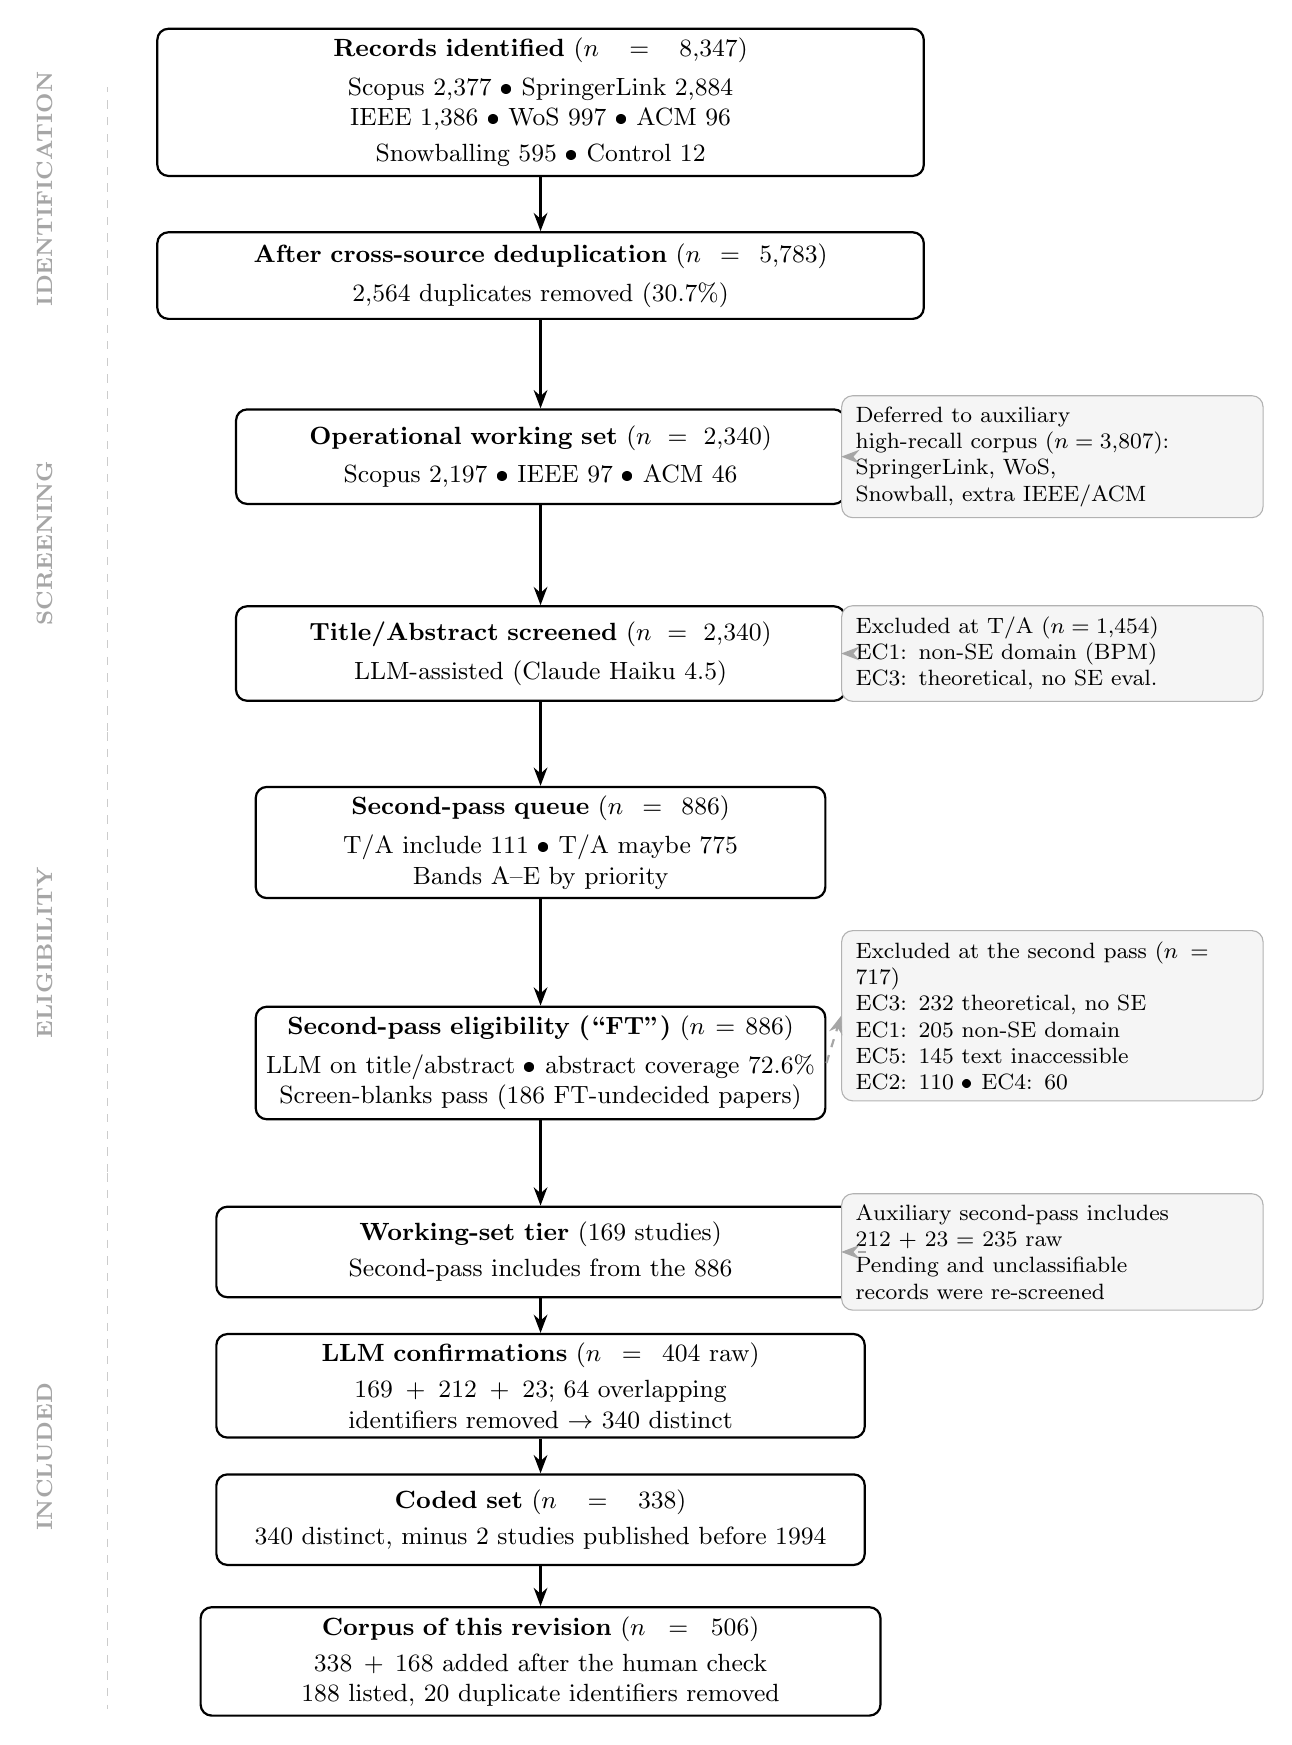
\begin{tikzpicture}[
  %% Main flow boxes (centre column) --- progressively narrower for funnel feel
  stg/.style={draw, rounded corners=4pt, align=center,
              text width=#1, minimum height=1.1cm,
              font=\small, fill=white, thick},
  stg/.default=8cm,
  %% Exclusion / note boxes (right column)
  exc/.style={draw, rounded corners=4pt, align=left,
              inner xsep=5pt, inner ysep=4pt,
              text width=5.0cm, minimum height=0.9cm,
              font=\footnotesize, fill=gray!8, draw=gray!60},
  %% Phase labels (left column)
  lbl/.style={font=\footnotesize\bfseries, text=gray!70,
              rotate=90, anchor=center},
  arr/.style={->, >=Stealth, thick},
  sidearr/.style={->, >=Stealth, dashed, draw=gray!70, thick},
]

%% -- PHASE: IDENTIFICATION ----------------------------------------------

\node[lbl] at (-6.8,-1.1) {IDENTIFICATION};
\draw[gray!40, dashed] (-6.0,-2.4) -- (-6.0, 0.2);

\node[stg=9.5cm, minimum height=1.3cm] (id) at (-0.5,0)
  {\textbf{Records identified} ($n = 8{,}347$)\\[3pt]
   Scopus~2{,}377 \textbullet{} \mbox{SpringerLink}~2{,}884\\
   IEEE~1{,}386 \textbullet{} WoS~997 \textbullet{} ACM~96\\[2pt]
   Snowballing~595 \textbullet{} Control~12};

\node[stg=9.5cm] (dedup) at (-0.5,-2.2)
  {\textbf{After cross-source deduplication} ($n = 5{,}783$)\\[3pt]
   2{,}564 duplicates removed (30.7\%)};

\draw[arr] (id) -- (dedup);

%% -- PHASE: SCREENING ----------------------------------------------------

\node[lbl] at (-6.8,-5.6) {SCREENING};
\draw[gray!40, dashed] (-6.0,-2.4) -- (-6.0,-8.0);

\node[stg=7.5cm, minimum height=1.2cm] (ws) at (-0.5,-4.5)
  {\textbf{Operational working set} ($n = 2{,}340$)\\[3pt]
   Scopus~2{,}197 \textbullet{} IEEE~97 \textbullet{} ACM~46};

\node[exc] (wsdrop) at (6.0,-4.5)
  {Deferred to auxiliary\\high-recall corpus ($n = 3{,}807$):\\
   \mbox{SpringerLink}, WoS,\\Snowball, extra IEEE/ACM};

\draw[arr] (dedup) -- (ws);
\draw[sidearr] (ws.east) -- (wsdrop.west);

\node[stg=7.5cm, minimum height=1.2cm] (ta) at (-0.5,-7.0)
  {\textbf{Title/Abstract screened} ($n = 2{,}340$)\\[3pt]
   LLM-assisted (Claude Haiku 4.5)};

\node[exc] (taexc) at (6.0,-7.0)
  {Excluded at T/A ($n = 1{,}454$)\\
   EC1: non-SE domain (BPM)\\
   EC3: theoretical, no SE eval.};

\draw[arr] (ws) -- (ta);
\draw[sidearr] (ta.east) -- (taexc.west);

%% -- PHASE: ELIGIBILITY --------------------------------------------------

\node[lbl] at (-6.8,-10.8) {ELIGIBILITY};
\draw[gray!40, dashed] (-6.0,-8.0) -- (-6.0,-13.6);

\node[stg=7cm, minimum height=1.3cm] (ftq) at (-0.5,-9.4)
  {\textbf{Second-pass queue} ($n = 886$)\\[3pt]
   T/A include~111 \textbullet{} T/A maybe~775\\
   Bands~A--E by priority};

\draw[arr] (ta) -- (ftq);

\node[stg=7cm, minimum height=1.4cm] (ft) at (-0.5,-12.2)
  {\textbf{Second-pass eligibility (``FT'')} ($n = 886$)\\[3pt]
   LLM on title/abstract \textbullet{} abstract coverage 72.6\%\\
   Screen-blanks pass (186 FT-undecided papers)};

\node[exc] (ftexc) at (6.0,-11.6)
  {Excluded at the second pass ($n = 717$)\\
   EC3: 232 theoretical, no SE\\
   EC1: 205 non-SE domain\\
   EC5: 145 text inaccessible\\
   EC2: 110 \textbullet{} EC4: 60};

\draw[arr] (ftq) -- (ft);
\draw[sidearr] (ft.east) -- (ftexc.west);

%% -- PHASE: INCLUDED ----------------------------------------------------

\node[lbl] at (-6.8,-17.2) {INCLUDED};
\draw[gray!40, dashed] (-6.0,-13.6) -- (-6.0,-20.4);

\node[stg=8cm, minimum height=1.15cm] (wsinc) at (-0.5,-14.6)
  {\textbf{Working-set tier} (169 studies)\\[2pt]
   Second-pass includes from the 886};

\node[exc] (auxinc) at (6.0,-14.6)
  {Auxiliary second-pass includes\\
   212 + 23 = 235 raw\\
   Pending and unclassifiable\\
   records were re-screened};

\draw[arr] (ft) -- (wsinc);
\draw[sidearr] (wsinc.east) -- (auxinc.west);

\node[stg=8cm, minimum height=1.15cm] (raw) at (-0.5,-16.3)
  {\textbf{LLM confirmations} ($n = 404$ raw)\\[2pt]
   $169 + 212 + 23$; 64 overlapping identifiers removed $\rightarrow$ 340 distinct};

\draw[arr] (wsinc) -- (raw);

\node[stg=8cm, minimum height=1.15cm] (coded) at (-0.5,-18.0)
  {\textbf{Coded set} ($n = 338$)\\[2pt]
   340 distinct, minus 2 studies published before 1994};

\draw[arr] (raw) -- (coded);

\node[stg=8.4cm, minimum height=1.25cm] (inc) at (-0.5,-19.8)
  {\textbf{Corpus of this revision} ($n = 506$)\\[2pt]
   $338 + 168$ added after the human check\\
   188 listed, 20 duplicate identifiers removed};

\draw[arr] (coded) -- (inc);

\end{tikzpicture}
\caption{PRISMA 2020 flow of the study selection. The included phase
  continues through the auxiliary screen, the removal of overlapping
  identifiers, the removal of two pre-1994 studies, and the human re-screen.
  The mapped set is 506 studies (Table~\ref{tab:ledger}). The 318-study
joint tables are an older cut (381 records minus 63 duplicates) and are
not a node of this flow. In the original run, 595 records with no abstract
and 16 records that stayed pending were closed under EC5; this revision
re-screened those records.}
\label{fig:prisma}
\end{figure}


\section{Results and Synthesis}
\label{sec:slr-synthesis}

\subsection{Overview of Included Studies}

This revision includes \textbf{506 studies}: 338 already coded, plus 168
added after the human check.

The 338 are the LLM list of 340 studies, minus two papers from 1991 and
1992. The 168 are what remains of 188 records the re-screen marked as
eligible, after 20 records that repeated a study already in the list were
removed. Eleven of the 168 were read as a PDF, 80 from the abstract, and
77 from the title only.

The three technique families were marked on \textbf{429} of the 506: the
338, plus the 91 added studies that had an abstract or a PDF. One of those
429, PRIMAD, has all three families. The 77 studies known only by the title
were left blank.

Table~\ref{tab:ledger} is the single count of every cut used in the
paper. Four of those rows answer different questions, and they are not
interchangeable. The context set is the 506: a study entered when it met
one of IC4a--IC4d. The rows with technique-family codes filled before this
round are the 338. The rows whose three family marks were filled, including
the 91 added studies read from an abstract or a PDF, are the 429. The
intersection of process mining, a stochastic model, and forecasting is one
study inside that 429. Each research question is answered on the cut named
in its sentence. The working-set tables, including the integration levels,
use 169 of the 338. The joint tables use 318. That 318 is what remained
after 63 duplicate records were removed from an earlier combined list of
381. The 340 is what remained after 64 duplicate records were removed from
404 raw confirmations. The two cuts were built by different removals.
Adding the 23 studies of the second auxiliary pass to 318 does not produce
340. The 8\% of suggested labels that the two reviewers did not accept is
not listed record by record, so the 506 still contains every suggested
include. Appendix~\ref{app:included} lists the 506 studies and groups them
by family.

\begin{table}[htbp]
\centering
\caption{Counts used in this paper. Each row is a different cut.}
\label{tab:ledger}
\small
\begin{tabular}{lp{8.1cm}}
\toprule
\textbf{Studies} & \textbf{Meaning} \\
\midrule
8{,}347 & Records retrieved, before deduplication. \\
5{,}783 & Records after deduplication. \\
2{,}340 & Working set screened (Scopus, IEEE, ACM). \\
3{,}807 & Auxiliary set screened. \\
404 & Raw LLM confirmations (169 + 212 + 23). \\
340 & Distinct LLM list (404 minus 64 duplicate records). \\
338 & The 340 minus two papers from 1991 and 1992. \\
381 & Earlier combined list, before the 318 cut. \\
318 & Joint tables (381 minus 63 duplicate records). Not 340 minus 23. \\
506 & This revision (338 + 168). \\
429 & Three family marks filled (338 + 91). \\
77 & Added studies known only by the title. Marks left blank. \\
\bottomrule
\end{tabular}
\end{table}

The list is \texttt{included\_studies\_506.csv}. The file of 340 rows is
kept so the removal of the two pre-1994 papers can be checked. Forty-three
of the 168 added studies were assigned a model score of at least 4/8. A
score taken from an abstract is not a quality assessment of the study, and
no score is used to keep or drop a study. The percentages in F1--F5, apart
from the count of one study in 429, use the 338 and the smaller cuts of
169 and 318. Those percentages were not re-marked by a human in this
revision.

The 169-study working-set tier spans 1995--2026 (publications dated 2026
that were already indexed on 12~April~2026 are retained), with a clear
acceleration from 2014 onward (Figure~\ref{fig:year-dist}). Sixty-nine
percent of working-set papers (117/169) appeared in 2015--2026.
A completed SEGRESS~\cite{kitchenham2023segress} reporting checklist is in
Appendix~\ref{app:segress}.

\begin{figure}[htbp]
\centering
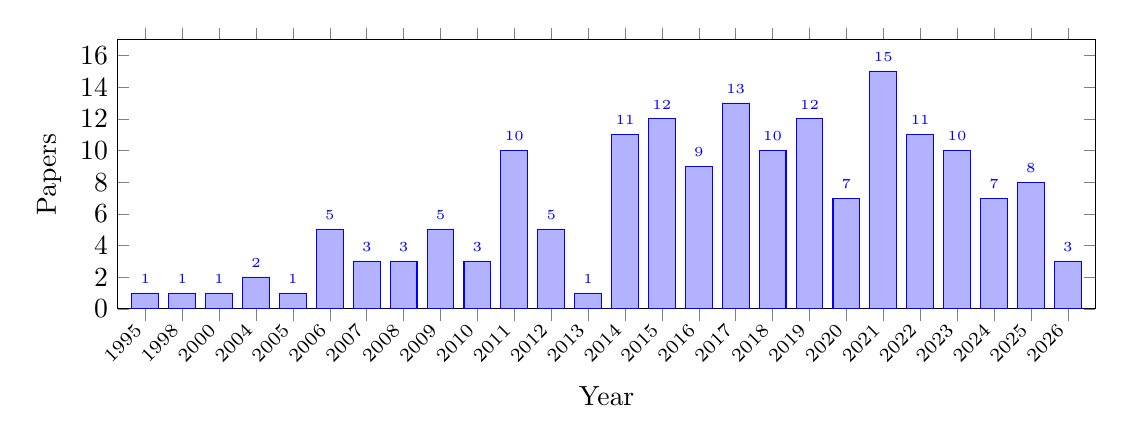
\begin{tikzpicture}
\begin{axis}[
  ybar,
  bar width=0.34cm,
  width=14cm, height=5cm,
  xlabel={Year},
  ylabel={Papers},
  xtick=data,
  xticklabels={1995,1998,2000,2004,2005,2006,2007,2008,2009,2010,2011,2012,2013,2014,2015,2016,2017,2018,2019,2020,2021,2022,2023,2024,2025,2026},
  x tick label style={rotate=45, anchor=east, font=\scriptsize},
  ymin=0, ymax=17,
  ytick={0,2,4,6,8,10,12,14,16},
  enlarge x limits=0.03,
  fill=gray!40,
  draw=black,
  nodes near coords,
  nodes near coords style={font=\tiny, above},
]
\addplot coordinates {
  (1,1)(2,1)(3,1)(4,2)(5,1)(6,5)(7,3)(8,3)(9,5)(10,3)(11,10)(12,5)(13,1)(14,11)(15,12)(16,9)(17,13)(18,10)(19,12)(20,7)(21,15)(22,11)(23,10)(24,7)(25,8)(26,3)
};
\end{axis}
\end{tikzpicture}
\caption{Publication year of the 169 working-set studies.}
\label{fig:year-dist}
\end{figure}

By document type, the majority are conference papers and journal articles.
By source database, Scopus is the dominant contributor, followed by
IEEE~Xplore and ACM~DL. Data extraction was completed for all 169 studies
using a structured LLM-assisted pipeline (\textit{claude-haiku-4-5-20251001})
operating on locally available PDFs (75/169, of which 73 were operationally
coded in the triangulation subset) or abstract/title metadata (94/169).

\subsection{Inclusion Criterion Coverage}

Figure~\ref{fig:ic-dist} shows the distribution of inclusion criteria among
the 169 working-set studies (criteria are non-exclusive; a paper may satisfy
multiple).

\begin{figure}[htbp]
\centering
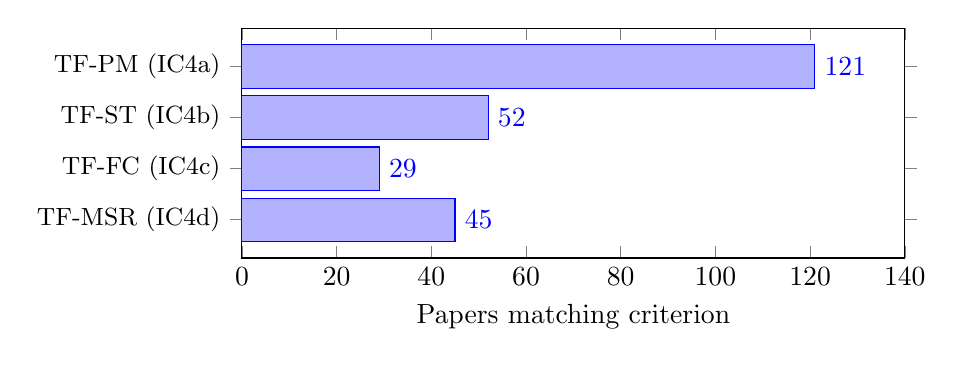
\begin{tikzpicture}
\begin{axis}[
  xbar,
  bar width=0.55cm,
  width=10cm, height=4.5cm,
  xlabel={Papers matching criterion},
  symbolic y coords={TF-MSR (IC4d), TF-FC (IC4c), TF-ST (IC4b), TF-PM (IC4a)},
  ytick=data,
  y tick label style={font=\small},
  xmin=0, xmax=140,
  nodes near coords,
  nodes near coords align={horizontal},
  fill=gray!40,
  draw=black,
  enlarge y limits=0.25,
]
\addplot coordinates {
  (121,{TF-PM (IC4a)})
  (52,{TF-ST (IC4b)})
  (29,{TF-FC (IC4c)})
  (45,{TF-MSR (IC4d)})
};
\end{axis}
\end{tikzpicture}
\caption{Inclusion criteria matched by the 169 working-set studies. Counts
are non-exclusive. TF-PM, TF-ST, TF-FC, and TF-MSR are the content criteria
IC4a--IC4d.}
\label{fig:ic-dist}
\end{figure}

TF-PM (process mining applied to SE artifacts) is the dominant criterion,
matched by 121 papers (71.6\%). TF-MSR (repository mining for process modeling)
is second at 45 papers (26.6\%), reflecting the MSR community's overlapping
contributions. TF-ST (stochastic modeling) appears in 52 papers (30.8\%) and
TF-FC (forecasting of process metrics) in 29 papers (17.2\%). Notably, 68
papers (40.2\%) match TF-PM only, without stochastic or forecasting components.
That split is the family-code count labeled F1 below. It was not re-marked
in this revision, and it is a count on these 169 studies.

\subsection{Prevalent Exclusion Patterns}

Among the 717 FT-excluded papers (Table~\ref{tab:ft-screening}), the largest
exclusion reason is EC3 (algorithmic or theoretical contribution without
software-engineering evaluation, $n=232$), indicating a substantial body of
process mining and stochastic modeling research that has not been empirically
applied to software engineering contexts. EC1 (domain exclusively outside
software development, $n=205$) is the second-largest reason and consists
primarily of generic business process management (BPM) studies that use the
same terminology as the search strings but apply techniques to organizational
processes unrelated to SDLC. EC5 (full text inaccessible, active post-audit
$n=145$; original historical stratum $n=148$) closes the group of large
strata, followed by EC2 (software as implementation platform
rather than analyzed process, $n=110$) and EC4 (out-of-scope secondary study,
$n=60$). EC counts are non-exclusive: the sum of per-EC counts
($232+205+145+110+60 = 752$) exceeds the 717 excluded papers by 35,
corresponding to papers that triggered more than one EC simultaneously. EC3
and EC1 are the two largest reasons in this exclusion list. That is a
property of the list. It does not confirm F3 or F4. Those labels, below,
are family-code counts on the 169 and the 318, and they were not re-marked
in this revision.

\subsection{Full-Text Extraction and PDF-Based Triangulation}
\label{sec:slr-pdf-enrichment}

Structured data extraction was performed on the full 169-study set using the
extraction template defined in Table~\ref{tab:extraction}. For each study,
the LLM extracted the research question, study type, research contribution,
PM technique, stochastic technique, software artifact, software process, data
source, dataset availability, tool used, main finding, limitations, and
replication-package status. Title-and-abstract metadata was used as the
primary input for studies without locally available PDFs (94/169); for the
remaining 75/169 studies a locally accessible PDF was available and used to
triangulate against the LLM-extracted fields. Of these 75 PDFs, 73 were
fully coded in the operational triangulation spreadsheet used for the
figures and positioning tables below.

The 73-paper PDF triangulation subset is therefore not a separate selection
stage and does not override the PRISMA counts. It does not confirm the
fields behind F1--F5. On 31 studies the exact match between a human rater
and the model on the free-text fields is 0\%. F1, F3, and F4 were not
re-marked in this revision.

Figure~\ref{fig:pdf-decision-dist} summarizes the operational triage profile
of the 73 coded PDFs (54 confirm-include, 13 confirm-include with
caveats, 6 confirm-exclude after full-text inspection); the formal selection
decisions reported in the PRISMA flow (Figure~\ref{fig:prisma}) are
unchanged.

\begin{figure}[tbp]
\centering
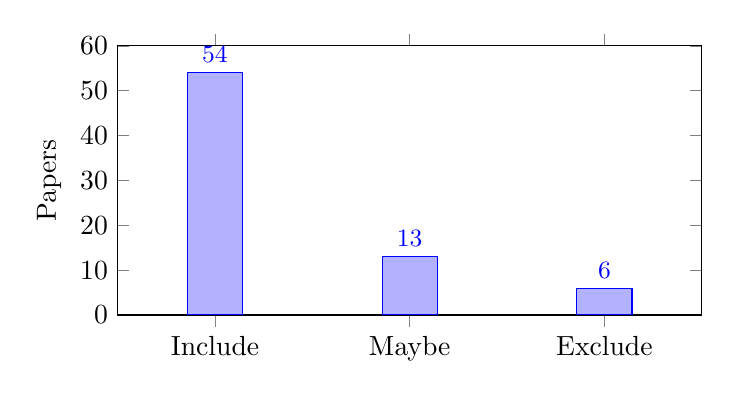
\begin{tikzpicture}
\begin{axis}[
  ybar,
  bar width=0.7cm,
  width=9cm, height=5cm,
  ylabel={Papers},
  symbolic x coords={Include,Maybe,Exclude},
  xtick=data,
  ymin=0, ymax=60,
  ytick={0,10,20,30,40,50,60},
  nodes near coords,
  nodes near coords style={font=\small, above},
  fill=gray!45,
  draw=black,
  enlarge x limits=0.25,
]
\addplot coordinates {(Include,54) (Maybe,13) (Exclude,6)};
\end{axis}
\end{tikzpicture}
\caption{Operational decision distribution in the 73-paper PDF triangulation subset.}
\label{fig:pdf-decision-dist}
\end{figure}

\subsection{RQ1: Application Landscape}
\label{sec:slr-rq1}

\subsubsection{RQ1.1: SDLC Phases Covered}

The model extraction of the 169 working-set studies, which this revision
did not re-mark, assigns SDLC phases as follows. It is not a description
of the 506. \textbf{Development activities} (coding,
commits, pull requests, repository evolution) dominate at 133 papers
(78.7\%); \textbf{quality-related activities} (testing, defect handling, code
review, process evaluation) appear in 74 papers (43.8\%);
\textbf{maintenance} appears in 38 papers (22.5\%);
\textbf{requirements engineering} in only 22 papers (13.0\%); and
\textbf{delivery/DevOps contexts} (CI/CD, build and release pipelines) in
just 18 papers (10.7\%). \textbf{Design and architecture} are not the primary
focus of any extracted study, and only 3 papers (1.8\%) center the analysis
on project management.

These 169 codes were not re-marked in this revision. They concentrate on
phases where digital traces are abundant and already timestamped, such as
commits, issues, test events, and pipeline executions. The early SDLC phases
are uncommon in these codes.

\subsubsection{RQ1.2: Event Log Sources and Construction}

Across the 169-study set, event logs are constructed primarily from four
source families: \textbf{version-control repositories} (Git/GitHub/SVN
commits) appear in 84 papers (49.7\%); \textbf{issue tracking systems}
(especially Jira and GitHub Issues) in 37 papers (21.9\%); \textbf{IDE
interaction logs} in 22 papers (13.0\%); and \textbf{CI/CD or build
pipelines} in 15 papers (8.9\%). The common pattern is not a native event
log but rather a \emph{derived} event log assembled from repository metadata,
commit histories, issue transitions, and (where available) pipeline records.

The dominant construction problem is case correlation across tools. Studies
frequently analyze one source in isolation or perform ad hoc joins between
issues and commits. In these 169 codes, that construction is rarely
explicit. The count is the model extraction labeled F2 below. A human
re-read did not confirm it: exact agreement on the free-text fields is
0\% on 31 studies.

A non-trivial fraction of studies report data sources only in coarse terms
(\textit{repository data}, \textit{VCS history}, \textit{open-source
projects}) without naming specific projects, time windows, or extraction
queries. Across the 169-study set, only 25 papers (14.8\%) explicitly state
that their dataset is publicly available and only 4 papers (2.4\%) declare a
replication package. These 25 and 4 are the same model count. They are
not a measure of incomplete reporting in the literature.

A complementary body of work constructs Markov models directly from GitHub
repository traces, bypassing explicit process discovery in favour of manual
state-space definition. Jo et al.\ \cite{jo2023} modelled developer activities
in GitHub repositories as Discrete-Time Markov Chains (DTMCs), finding that
commits account for 62.73\% of long-term activity, and employed probabilistic
temporal logic to extract collaboration patterns relevant to project management.
This approach was extended in \cite{jo2024}, where Probabilistic Model Checking
with Computation Tree Logic was applied across five repositories to characterise
temporal dynamics, state-transition probabilities, and key behavioural drivers,
yielding transparent and explainable project forecasts. Ortu et al.\ \cite{ortu2023}
complemented these structural analyses by combining Markov chains with social
network analysis to identify fault-insertion and fault-fixing behavioural patterns
across Apache Software Foundation projects, demonstrating that developer expertise
significantly moderates defect introduction likelihood. Collectively, these studies
confirm that SDLC event logs extracted from public repositories are sufficiently
rich to support state-transition modelling. However, the event-to-state mapping
adopted across these works is defined manually and differs from study to study;
none derives the state space from a discovered process model.


\subsection{RQ2: Techniques and Prediction}
\label{sec:slr-rq2}

\subsubsection{RQ2.1: Discovery Algorithms Applied to SDLC}

The canonical origin of process mining applied to software development contexts
can be traced directly to the foundational contributions of Cook and Wolf in the
mid-1990s. In their seminal work, \cite{cook1995} introduced three automated
process discovery methods---algorithmic grammar inference, Markov models, and
neural networks---demonstrating that finite-state machine representations of
software processes could be extracted automatically from event traces,
substantially lowering the barrier to formal process modeling. This line of
inquiry was consolidated in \cite{cook1998}, which refined the event-based
discovery methodology and established the conceptual vocabulary of inferring
workflow structures from historical execution data, a paradigm that remains
central to the field today. Notably, both contributions embedded stochastic
reasoning---particularly Markov chain representations---within the discovery
pipeline, anticipating the probabilistic extensions that would later characterise
mature process mining frameworks. The translation of these principles into an
explicit, named framework for software engineering contexts was accomplished by
\cite{rubin2007}, who applied the ProM toolkit to source code management logs
and demonstrated multi-perspective analysis spanning control-flow, informational,
and organisational dimensions. Together, these three works constitute the seminal
arc of TF-PM, establishing automated discovery from SDLC event logs as both
technically feasible and analytically productive.

The family-code count on the 169 working-set studies, which this revision
did not re-mark, has 121 studies (71.6\%) matching TF-PM in the form of
discovery, conformance checking, or process-oriented repository analysis.
The same count has 29 papers (17.2\%) matching TF-FC. It is not a
description of the literature. At the technique level, the model names the
\textbf{inductive miner} in 51 papers, the \textbf{alpha miner} in 45, \textbf{conformance checking} in 30,
and the \textbf{heuristic miner} in 22; 11 papers are coded as social
network analysis on developer interactions. Those names were not
re-extracted in this revision.

The same family-code count names an explicit stochastic technique in 52 of
169 studies (30.8\%): 38 papers (22.5\%) use Markov chains, 15 (8.9\%) use
Monte Carlo simulation, 9 (5.3\%) use stochastic Petri nets, and 8 (4.7\%)
use system dynamics. Those technique counts are non-exclusive. The
extraction also records 110 rows without a stochastic component and 29 rows
with stochastic methods in an auxiliary role. These are the original codes
on this cut. They were not re-marked in this revision, and they are not a
description of the forecasting literature, as shown in
Figure~\ref{fig:pdf-technique-dist}.

\begin{figure}[tbp]
\centering
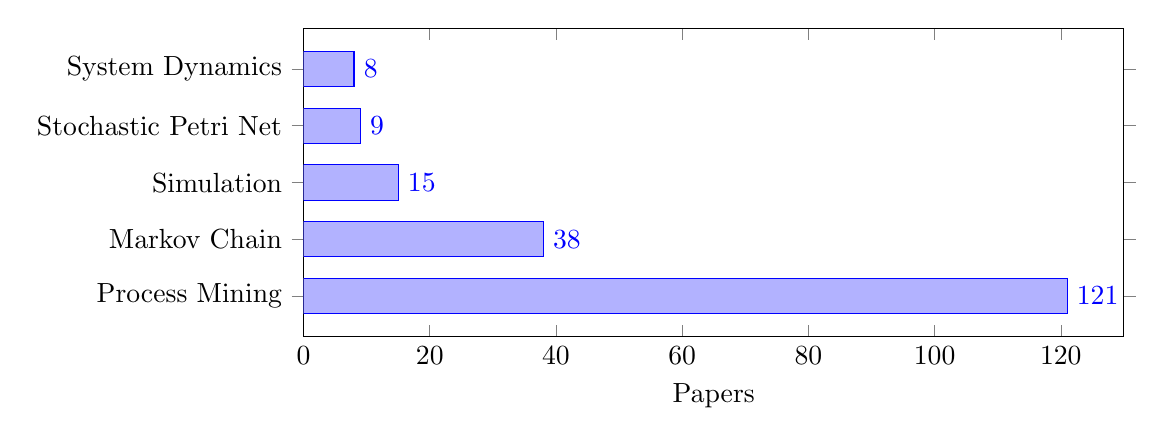
\begin{tikzpicture}
\begin{axis}[
  xbar,
  bar width=0.45cm,
  width=12cm, height=5.5cm,
  xlabel={Papers},
  symbolic y coords={Process Mining,Markov Chain,Simulation,Stochastic Petri Net,System Dynamics},
  ytick=data,
  xmin=0, xmax=130,
  nodes near coords,
  nodes near coords align={horizontal},
  fill=gray!45,
  draw=black,
  enlarge y limits=0.18,
]
\addplot coordinates {
  (121,{Process Mining})
  (38,{Markov Chain})
  (15,{Simulation})
  (9,{Stochastic Petri Net})
  (8,{System Dynamics})
};
\end{axis}
\end{tikzpicture}
\caption{Main technique families in the 169 working-set studies.
Counts are non-exclusive: a paper may use multiple technique families.
These counts were not re-marked in this revision.}
\label{fig:pdf-technique-dist}
\end{figure}

\subsubsection{RQ2.2: Predictive and Stochastic Techniques}

Three distinct sub-families of stochastic techniques emerge from the confirmed
literature. The first, \textbf{Markov-chain-based prediction}, encompasses
models that represent software processes as discrete state transitions, including
reinforcement learning agents grounded in Markov Decision Processes for
pull-request outcome prediction \cite{joshi2024}, probabilistic risk
quantification from repository data \cite{jeon2015}, defect removal
effectiveness under code churn \cite{tian2005}, agile state-space planning and
tracking \cite{tyagi2021}, release-time forecasting via generalised reliability
models \cite{washizaki2015}, and Stochastic Automata Networks for Waterfall team
estimation \cite{massitela2018}. The second sub-family, \textbf{stochastic
Petri nets}, models concurrency and asynchrony in DevOps and CI/CD pipelines
through non-Markovian specifications \cite{benmesmia2021} and sensitivity
analyses that identify bottleneck stages governing delivery probability
\cite{bhadra2022,bhadra2023}. The third sub-family, \textbf{Monte Carlo
simulation}, drives project-level forecasting in hybrid System Dynamics models
\cite{li2020}, agile risk assessment frameworks \cite{lunesu2021}, cycle-time
economic analysis \cite{magennis2015}, and the PRIMAD digital-twin architecture
for SDLC \cite{guinea2025}.

Despite their methodological diversity, the cited descriptions share a
parametrisation pattern. Transition
probabilities, firing rates, and distributional parameters in these
descriptions come from aggregate project statistics---historical defect
counts, phase-level duration averages, or summary velocity metrics---rather
than from transition frequencies extracted through process mining of
fine-grained event logs \cite{nafreen2020,bhadra2022,li2020}. In the same
descriptions, model states stay anchored to coarse lifecycle phases. This
is a reading of those descriptions. It is not a re-mark of the family codes
labeled F3, which remain the original counts on the 169 and the 318.

Three studies exemplify the productive convergence of process mining and
stochastic modelling at the component level. Incerto~\cite{incerto2025}
demonstrated that variable-length Markov chains outperform eighteen existing
stochastic conformance-checking techniques across ten of eleven benchmark
datasets, establishing that higher-order sequential dependencies in event logs
can be captured without sacrificing computational tractability.
L\'opez-Pintado~\cite{lopezpintado2023} extended process-simulation fidelity by
replacing deterministic resource-availability calendars with probabilistic
counterparts discovered directly from event logs, showing that stochastic
resource representations more accurately replicate empirical cycle-time
distributions. Jalote~\cite{jalote2021} took a complementary perspective,
modelling programmer task sequences as first-order Markov chains derived from
IDE interaction logs and demonstrating that transferring the process patterns of
high-productivity developers to average-productivity peers yields measurable
productivity gains. In the studies cited in this paragraph, the stochastic
layer stays on one analytical concern. That reading does not establish a
unified forecasting pipeline in the literature.

The closest published work to a fully integrated multi-stage architecture is
PRIMAD, proposed by Guinea-Cabrera~\cite{guinea2025}, which orchestrates
pm4py-based process discovery, Akka actor-system simulation, and LightGBM
supervised learning within an evolutionary Digital Twin framework for the SDLC.
Nevertheless, PRIMAD remains at what may be characterised as Level~2 integration:
validation is reported per component rather than across the assembled pipeline,
no formal inter-stage contracts govern the handoffs between discovery,
simulation, and learning modules, and the architecture incorporates no dedicated
Monte Carlo forecasting layer capable of propagating uncertainty estimates
end-to-end. On the family codes filled for the 429 studies, PRIMAD is the
one row that matches the three families. The 338 were not re-marked in this
revision. None of the 91 added studies read from an abstract or a PDF adds
a second triple. The 77 title-only studies are outside that count. A single
code on that cut is not a statement that the literature contains no
end-to-end pipeline.

Studies that combine process mining with forecasting objectives (TF-PM~$\cap$~TF-FC)
tend to approach prediction through \emph{process enhancement} rather than
through explicit stochastic modelling. Gupta~\cite{gupta2017} demonstrated that
combining inductive miner discovery with Markov chain-based predictive analytics
enables identification of recurring failure patterns in software maintenance
workflows. Pourbafrani et al.~\cite{pourbafrani2021} presented SIMPT, a tool
that extracts process trees with time parameters from event logs and enables
interactive what-if simulation; its successor work~\cite{buliga2025} further
integrates generative AI with business process simulation to produce
conformance-preserving what-if scenarios. Caldeira et al.~\cite{caldeira2022}
mine IDE interaction logs and show that process complexity metrics derived from
ProM correlate moderately ($r \approx 0.43$) with software cyclomatic
complexity, achieving predictive accuracies exceeding 92\%, demonstrating the
feasibility of process-derived features for product-quality prediction.

Taken together, the papers cited in this paragraph describe PM output feeding
a downstream model. That reading is not a census of the SE literature. None of
these cited systems is described as reporting a probability distribution
over completion time or remaining steps for an individual process instance.


\subsection{RQ3: Integration and Gaps}
\label{sec:slr-rq3}

\subsubsection{RQ3.1: PM and Stochastic Integration Level}

The original family codes on the 169 working-set studies, which this
revision did not re-mark, place rows on the L0--L3 scale defined in
Table~\ref{tab:positioning}: the number of technique families TF-PM, TF-ST,
and TF-FC a study matches. The
largest two-family cluster, comprising papers that touch TF-ST and TF-FC
without TF-PM---including stochastic Petri net models of CI/CD pipelines
\cite{bhadra2022,bhadra2023}, Markov-based project estimation
\cite{massitela2018,tyagi2021}, and Monte Carlo risk simulation
\cite{lunesu2021,magennis2015}---is coded \textbf{L1},
applying stochastic modelling to software processes without any process
discovery layer. Papers spanning TF-PM and TF-ST, such as the VLMC conformance
checker of \cite{incerto2025} and the probabilistic resource-calendar discoverer
of \cite{lopezpintado2023}, are also coded \textbf{L1}: they couple discovered
process structure with stochastic reasoning, but neither closes the loop
toward distributional schedule forecasting. Papers combining TF-PM with TF-FC, such as
\cite{gupta2017} and \cite{caldeira2022}, use process mining descriptively to
assess workflows but lack the stochastic machinery required for Monte Carlo
distributional forecasts. The PRIMAD framework \cite{guinea2025} is the one
triple match in these codes. It assembles event-log discovery,
simulation, and ML prediction, and its evaluation is described as component-wise,
so the code is L2 rather than a validated end-to-end contract. No row
in these 169 codes is \textbf{L3}. L3 would be a row that matches the three
families and states formal interfaces validated end-to-end on SDLC event logs.
These codes do not establish that no such architecture exists in the literature.

The same 169 codes, not a confirmation of a literature pattern, are as follows. 
1 of 169 papers (0.6\%) jointly satisfies TF-PM, TF-ST, and TF-FC,
and that paper's extraction does not record a formal end-to-end
pipeline contract. Pairwise codes are TF-PM$\cap$TF-ST in 10 papers (5.9\%), TF-PM$\cap$TF-FC
in 7 papers (4.1\%), and TF-ST$\cap$TF-FC in 18
papers (10.7\%). No row in these 169 codes is an
\textbf{L3} architecture. The same triple on the 318 joint tables is also one
paper. A rare code on these cuts is not a rare pattern in the literature. The
operational coding of the 73-PDF triangulation subset is a view of that subset and is summarized in
Figure~\ref{fig:pdf-integration-priority}.

\begin{figure}[p]
\centering
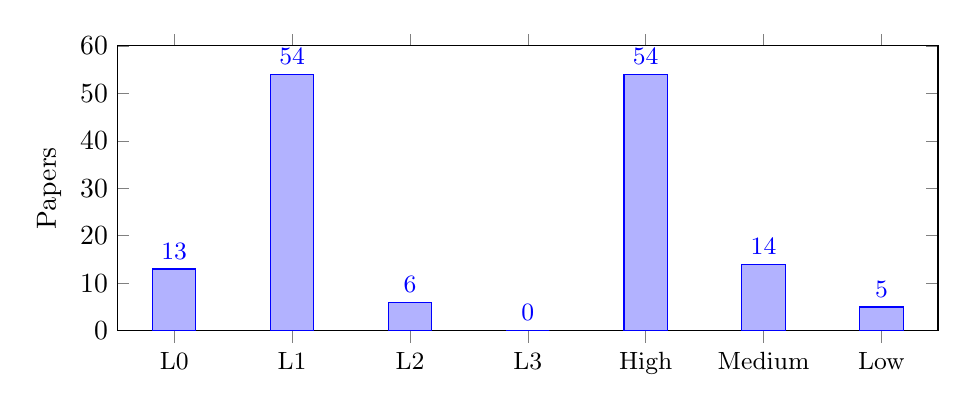
\begin{tikzpicture}
\begin{axis}[
  ybar,
  bar width=0.55cm,
  width=12cm, height=5.2cm,
  ylabel={Papers},
  symbolic x coords={L0,L1,L2,L3,High,Medium,Low},
  xtick=data,
  x tick label style={font=\small},
  ymin=0, ymax=60,
  ytick={0,10,20,30,40,50,60},
  nodes near coords,
  nodes near coords style={font=\small, above},
  fill=gray!45,
  draw=black,
  enlarge x limits=0.08,
]
\addplot coordinates {(L0,13) (L1,54) (L2,6) (L3,0) (High,54) (Medium,14) (Low,5)};
\end{axis}
\end{tikzpicture}
\caption{Operational integration levels and reading-priority distribution in the 73-paper PDF triangulation subset.}
\label{fig:pdf-integration-priority}
\end{figure}

\subsubsection{RQ3.2: Gap Analysis}

Three readings of the 169-study extraction follow. They were not re-marked
in this revision, and they are not a description of the literature.
First, the family-code count labeled F1: 121 papers (71.6\%) match process
mining and 29 (17.2\%) match forecasting of a process metric.
Second, the model assigned study types on these 169 rows: 69
(40.8\%) case studies, 34 (20.1\%) tool papers, 33 (19.5\%) theoretical,
13 (7.7\%) simulation-only, 10 (5.9\%) controlled experiments, 5 (3.0\%)
surveys, and 5 (3.0\%) residual categories (mixed, framework, exploratory;
sum: $69+34+33+13+10+5+5 = 169$). That assignment was not re-marked.
Third, the model count labeled F2: 25 of 169 papers (14.8\%) declare a
public dataset and 4 (2.4\%) declare a replication package. On 31 studies
the exact match between a human rater and the model on those free-text
fields is 0\%. The scores in Table~\ref{tab:qa-results} are what the same
model assigned. They do not confirm the count.

These readings do not establish that an end-to-end workflow is absent from
the literature. The evidence-type distribution in the 73-PDF subset
(Figure~\ref{fig:pdf-evidence-dist}) is a view of that subset. It is not a
separate selection layer, and it does not confirm the fields.

\begin{figure}[tbp]
\centering
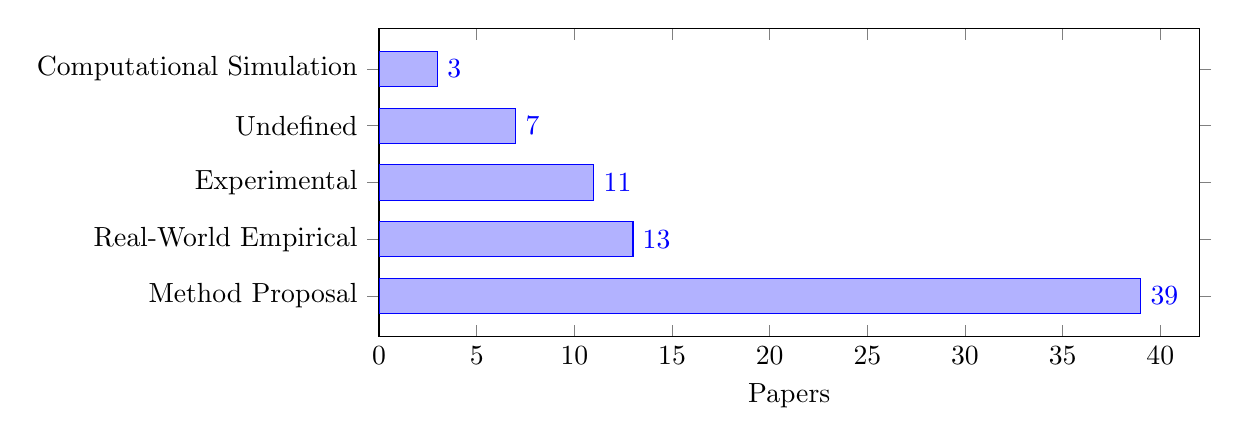
\begin{tikzpicture}
\begin{axis}[
  xbar,
  bar width=0.45cm,
  width=12cm, height=5.5cm,
  xlabel={Papers},
  symbolic y coords={Method Proposal,Real-World Empirical,Experimental,Undefined,Computational Simulation},
  ytick=data,
  xmin=0, xmax=42,
  nodes near coords,
  nodes near coords align={horizontal},
  fill=gray!45,
  draw=black,
  enlarge y limits=0.18,
]
\addplot coordinates {
  (39,{Method Proposal})
  (13,{Real-World Empirical})
  (11,{Experimental})
  (7,{Undefined})
  (3,{Computational Simulation})
};
\end{axis}
\end{tikzpicture}
\caption{Evidence-type distribution in the 73-paper PDF triangulation subset.}
\label{fig:pdf-evidence-dist}
\end{figure}


\section{Discussion}
\label{sec:slr-discussion}

\subsection{Research Gap Identification}
\label{sec:slr-gaps}

F1, F3, and F4 are family-code counts. Each sentence names its cut: 169,
318, or the 429 for the triple. None of those percentages is a rate over
the 506. F2 and F5 are counts extracted by the same model that screened
the papers. On 31 studies a human rater and the model had 0\% exact
agreement on those fields, so F2 and F5 are not confirmed findings.

\begin{description}

\item[F1: Descriptive ceiling (family codes on 169 and on 318).]
These percentages are the original family codes. They were not re-marked
by a human in this revision, and they are not a rate over the 506.
In the \textbf{working-set tier} (169 papers), 121 (71.6\%) match TF-PM
(process mining in SE) but only 29 (17.2\%) advance to TF-FC (forecasting
of process metrics). In the \textbf{combined analytical subset} (318 papers,
deduplicated), the proportion shifts because the auxiliary corpus pulled in
more stochastic-only and forecasting-only studies that did not employ
explicit process mining: 160 (50.3\%) match TF-PM, 100 (31.4\%) match TF-FC,
and 78 (24.5\%) match TF-PM alone. In both tiers the dominant contribution
type is discovery or conformance checking, not predictive analytics or
distributional forecasting; the descriptive ceiling identified in the
working-set tier persists in the combined tier.

\item[F2: Event-log construction (model count, not confirmed).]
These counts are model extractions. Exact agreement with a human rater on
the free-text fields is 0\% on the 31-study sample, and the fields were not
re-extracted by a human.
The same model count, on both cuts, is as follows. Working-set tier:
only 25 of 169 papers (14.8\%) declare the dataset as publicly available
and only 4 (2.4\%) declare any replication package. Combined analytical
subset: 44 of 318 papers (13.8\%) declare a public dataset and 9 (2.8\%)
declare a replication package. The model also records ad hoc joins between
version-control commits
(112 of 318 papers, 35.2\%), issue trackers (44, 13.8\%), Jira (46, 14.5\%),
GitHub (43, 13.5\%), and IDE interaction logs (37, 11.6\%). The quality
scores are assigned by the same model. They do not confirm this count.

\item[F3: Stochastic integration (family codes on 169 and on 318).]
These percentages are the original family codes. They were not re-marked
by a human in this revision.
Working-set tier: 52 of 169 papers (30.8\%) apply stochastic models
(TF-ST); 38 (22.5\%) Markov chains, 15 (8.9\%) Monte Carlo, 9 (5.3\%)
stochastic Petri nets, 8 (4.7\%) system dynamics; TF-ST$\cap$TF-FC covers 18
papers (10.7\%); TF-PM$\cap$TF-ST covers 10 (5.9\%). Combined analytical
subset: the
auxiliary corpus contributes a substantial number of stochastic-only papers
not previously surfaced by the working-set queries; 152 of 318 (47.8\%)
match TF-ST (with 86 Monte Carlo, 67 Markov, 54 system dynamics, 15 SPN), 81
(25.5\%) combine TF-ST with TF-FC (forecasting), and 13 (4.1\%) combine TF-ST
with TF-PM (process mining). On these codes, TF-PM$\cap$TF-ST is 10 of 169
(5.9\%) and 13 of 318 (4.1\%). The 318 codes contain more stochastic-only
rows than the 169 codes. That is a difference between the two cuts. It is
not a description of the stochastic literature, and it was not re-marked
in this revision. The largest second-pass exclusion in
the working-set queue is EC3 (232 of 886). That is a property of this
screen.

\item[F4: Pipeline fragmentation (family codes on 169, 318, and 429).]
These percentages are the original family codes on the 169 and the 318.
They were not re-marked by a human in this revision. The family marks
added in this revision are the 91 studies read from an abstract or a PDF.
None of those 91 has all three families.
No coded row in the 429 states a formal
PM $\rightarrow$ Markov $\rightarrow$ MC $\rightarrow$ ML contract with
inter-stage data contracts. That statement is about those rows.
Working-set tier (169 papers): the joint convergence
TF-PM$\cap$TF-ST$\cap$TF-FC appears in 1 paper (0.6\%), and that paper
does not specify a formal end-to-end pipeline contract; pairwise
convergences are TF-PM$\cap$TF-ST: 10 (5.9\%), TF-PM$\cap$TF-FC: 7 (4.1\%),
TF-ST$\cap$TF-FC: 18 (10.7\%). Combined analytical subset (318 papers,
deduplicated): TF-PM$\cap$TF-ST$\cap$TF-FC remains 1 paper (0.31\%), with pairwise
convergences TF-PM$\cap$TF-ST: 13 (4.1\%), TF-PM$\cap$TF-FC: 10 (3.1\%),
TF-ST$\cap$TF-FC: 81 (25.5\%). These counts describe the coded studies, not the 506-study corpus. Full-text
Recall on the working-set sample is 0.630 (29 of 46; Wilson 95\% CI
0.486--0.755). The screen missed eligible studies, so a rare pattern in the
338 is not a rare pattern in the literature.
PRIMAD \cite{guinea2025} is that one study inside the 429. It assembles discovery,
simulation, and learning components but validates each independently and
leaves the unified pipeline unevaluated. Its scope is SDLC-oriented: it builds a
digital twin from issue-tracking flows in JIRA. It combines empirical
process discovery (\texttt{pm4py}), a Python-based simulation core, an Akka
actor system, and supervised machine learning
for context-aware prediction. The reported results are component-wise:
the paper does not validate a coupled PM $\rightarrow$ stochastic
simulation $\rightarrow$ ML pipeline as one architecture.
The 77 added studies read from the title alone are outside this count.

\item[F5: Process-derived features (model count, not confirmed).]
These counts are model extractions of the research-contribution and
algorithm fields. They were not re-extracted by a human. On 31 studies the
exact match with a human rater on those fields is 0\%. A Scopus search on
31~October~2026 with machine-learning terms returned 165 records; title
screening left 19 IC4c includes, and none joins the three families
(Section~\ref{sec:slr-search}). Those 19 are not in the counts below.
The counts below are the studies the three original strings retrieved.
In those model counts, the coded ML/prediction rows rarely name a feature
taken from a process model. Working-set tier: 32
papers whose research contribution centers on ML/prediction; only 1
explicitly couples ML with a named process-mining algorithm (alpha,
inductive, heuristic, conformance, fuzzy, or Petri-net-based discovery).
Combined analytical subset: the auxiliary corpus added a large number of ML/prediction
papers (110 in the combined 318 set), but the rate of process-mining
coupling remains low: only 4 of 110 (3.6\%) jointly use a named PM
algorithm. Conformance scores, rework counts, Markov-expected remaining
time, and path entropy are absent from these model counts. They were not
re-extracted by a human, so their absence here is not an absence in the
literature.

\end{description}

These five statements are not a census of a confirmed corpus. F1, F3, and
F4 are the original family codes on the cut named in each sentence. They
were not re-marked in this revision. F2 and F5 are model extractions. On
31 studies the exact match with a human rater on those fields is 0\%, so
they are not confirmed. D1, D3, D5, and D4 name the same cuts. The agenda
in Section~\ref{sec:slr-agenda} uses those cuts as motivation. It does not
turn them into confirmed findings.


\subsection{Integration Levels}
\label{sec:slr-positioning}

Table~\ref{tab:positioning} defines the integration levels used throughout
the article and reports their counts. A level is determined only by how many
of the three \emph{technique} families a study matches (TF-PM, TF-ST,
TF-FC); TF-MSR describes the data source and is not counted. With this
single definition, the L1 and L2 rows coincide with the pairwise and triple
intersections reported under F3 and F4.

\begin{table}[htbp]
\centering
\caption{Integration levels of the 169 working-set studies. A level counts
how many of TF-PM, TF-ST, and TF-FC the study matches.}
\label{tab:positioning}
\small
\begin{tabularx}{\linewidth}{@{}c X r X@{}}
\toprule
\textbf{Level} & \textbf{Operational definition} & \textbf{Papers} & \textbf{Example} \\
\midrule
L0 & At most one technique family & 136 & Single-technique studies \\
L1 & Exactly two technique families (TF-PM$\cap$TF-ST: 9;
     TF-PM$\cap$TF-FC: 6; TF-ST$\cap$TF-FC: 17) & 32
   & Incerto~\cite{incerto2025}; L\'opez-Pintado~\cite{lopezpintado2023} \\
L2 & All three technique families (TF-PM$\cap$TF-ST$\cap$TF-FC) & 1
   & PRIMAD~\cite{guinea2025} \\
L3 & All three families coupled through explicit interfaces and validated
     end-to-end & 0 & --- \\
\midrule
\textbf{Total} & & \textbf{169} & \\
\bottomrule
\end{tabularx}

\smallskip
\footnotesize\textit{Note:} L1 counts exclude the single L2 study, so they are
one lower than the inclusive pairwise intersections in F3/F4 (10, 7, 18).
The 73-PDF operational coding (Figure~\ref{fig:pdf-integration-priority}) uses
a reading-based classification and is reported separately.
\end{table}

The authors' PATHCAST proposal is one candidate design for L3. It is
\textbf{not} evaluated in this mapping study and is listed only as a
research-agenda hypothesis motivated by F1--F5 (RA2--RA4,
Section~\ref{sec:slr-agenda}).


\subsection{Proposed Taxonomy: SPMF}
\label{sec:slr-taxonomy}

Based on the systematic analysis, this review proposes the Software Process
Mining and Forecasting (SPMF) taxonomy with three dimensions:

\begin{description}
\item[Analytical Depth] classifies studies along four levels (labelled AD
  to avoid confusion with the integration levels L0--L3): AD1
  (Descriptive: discovery, conformance), AD2 (Diagnostic: bottleneck, rework),
  AD3 (Predictive: outcome, remaining time), and AD4 (Forecasting:
  distributional, probabilistic).

\item[SDLC Coverage] maps which lifecycle phases are addressed: Requirements
  and Design, Development (coding, commits, PRs), Quality (testing, reviews,
  bugs), Delivery (CI/CD, release), and Operations (incidents, maintenance).

\item[Technique Integration] classifies methodological combination:
  Single (PM only, ML only, MC only), Dual (PM + ML, PM + Markov, Markov + MC),
  and Pipeline (PM $\rightarrow$ Markov $\rightarrow$ MC $\rightarrow$ ML).
\end{description}


\subsection{Research Agenda}
\label{sec:slr-agenda}

The gaps identified motivate four research directions:

\begin{description}
\item[RA1: Standardized Event Log Construction for SDLC.]
  The model count, which a human re-read did not confirm, is 25 of 169
  working-set papers declaring a public dataset. Target: frameworks for transforming
  heterogeneous repository data into comparable event logs with cross-tool
  case correlation.

\item[RA2: Process-Aware Stochastic Forecasting.]
  Motivated by F3: TF-ST$\cap$TF-FC reaches 18/169 (10.7\%) in the working set
  but TF-PM$\cap$TF-ST remains 10/169 (5.9\%). Target: formal integration of
  mined transition structure with Markov/Monte Carlo forecasting.

\item[RA3: Process-Derived Features for ML.]
  Motivated by F5: only 1/32 ML-centric working-set papers couples a named PM
  algorithm with prediction. Target: systematic use of conformance, rework,
  and path-entropy features in SE predictors.

\item[RA4: Empirical Benchmarking of Integrated Pipelines.]
  Motivated by F4: one study (PRIMAD) satisfies
  TF-PM$\cap$TF-ST$\cap$TF-FC among the 429 studies with family marks filled.
  The 77 title-only additions are not in that count. Target: comparable OSS
  benchmarks with temporal hold-out for end-to-end PM--stochastic--ML
  pipelines; formal specification and evaluation of candidates such as
  PATHCAST remain future work by the authors.
\end{description}


\subsection{Implications for Practitioners}
\label{sec:slr-practitioners}

These three points are readings of the 169 working-set codes. They were
not re-extracted by a human, and they are not a description of the 506.
First, in those codes, structured event logs in issue trackers are the
usual input to process mining. Second, the same codes name the inductive
miner in 51 papers and the alpha miner in 45 papers. Third, the stochastic
extension in those codes uses Markov chains and Monte Carlo on data the
studies already describe as present in the logs. The challenge those codes
describe is methodological composition.


\section{Threats to Validity}
\label{sec:slr-threats}

\subsection{Construct Validity}

The search strings may exclude studies that use non-canonical terminology.
This threat is mitigated through three mechanisms: the complementary MSR
string, the frontier stochastic-PM string, and one snowballing iteration
over 595 records attributed to 400 source DOIs
(Section~\ref{sec:slr-search}). The ten control papers were recovered, but
this is a weak check: they were known when the strings were written, so
their recovery does not bound the proportion of relevant studies the
strings miss. Those ten papers are not the snowballing seed list.

\subsection{Internal Validity}

LLM-based screening introduces the risk of systematic decision bias. We
report six aspects of how this risk was handled: (i)~structured outputs;
(ii)~author inspection of \texttt{include} decisions; (iii)~human
validation of the selection against a two-rater reference standard;
(iv)~LLM--LLM cross-model agreement; (v)~the T/A false-positive rate; and
(vi)~the closure rule for unresolved cases used in the original run.

(i)~\textbf{Structured outputs}. All screening responses use a strict JSON
schema, enabling post-hoc analysis of decision patterns and rationale
distributions.

(ii)~\textbf{Author inspection of LLM \texttt{include} decisions}.
Every paper retained at the FT stage of the original run was inspected by the
first author against the PRISMA flow before being added to the 169-study
working-set tier. The escalation set was judged by both reviewers
(Section~\ref{sec:slr-threats}).

(iii)~\textbf{Human validation of the selection}.
\emph{T/A stage.} A stratified random 20\% sample of working-set T/A
decisions ($n=468$) was screened by a human rater blind to the LLM. In the
working set, LLM \texttt{maybe} decisions were forwarded to FT screening
(Section~\ref{sec:slr-results-selection}); against the human labels, the
operational T/A Recall is therefore 72/72 $=1.000$ (Wilson 95\% CI
$0.949$--$1.000$). Counting \texttt{maybe} as a negative, as the R1
manuscript did, gives 18/72 $=0.250$, but that figure describes a decision
rule the working set never applied.

\emph{FT stage --- R1 reference standard withdrawn.} The FT reference
standard reported in R1 ($n=177$) did not record eligibility: all 126 human
\texttt{include} labels coincided with papers for which a PDF had been
obtained, and 50 of the 51 human \texttt{exclude} labels were annotated
``PDF not accessible''. The resulting Recall (0.246) measured PDF
availability, not screening error, and is withdrawn.

\emph{FT stage --- round-2 validation.} Before any new judgement we
pre-registered the check
(\texttt{PREREGISTRATION\_round2\_validation.md}; success if the point
estimate of Recall is at least 0.90). The same 177 records were judged
against Table~\ref{tab:criteria} by two raters, independently, blind to the
LLM and to each other. Disagreements were resolved by consensus. A record
whose text could not be obtained is \texttt{not\_assessable} and leaves the
denominator. Six records are in that class. Agreement between the raters,
before consensus, is $\kappa = 0.654$.

The reference standard is the consensus after a full-text re-reading of the
23 records the first consensus had included and the LLM had excluded. Five of
those 23 are ineligible. One is not assessable, because the file on disk is
a conference programme. Seventeen remain eligible. Against that reference the
LLM's full-text Recall is 0.630 (29 true positives out of 46 eligible
studies; Wilson 95\% CI 0.486--0.755). Lost evidence is 0.370. MCC is 0.656
and WMCC with false negatives weighted ten to one is 0.168
(Table~\ref{tab:r2-confusion}). The same Recall, 0.630, is obtained if the
second rater's labels are used alone. The first author had computed the
round-1 agreement report on this sample and may remember some LLM decisions.
The second rater had no such exposure. The result is below 0.90, so the
pre-registered rule required a human re-screen of the accessible working-set
records the LLM had excluded.

\emph{Auxiliary tier.} The same rule required a check of LLM non-includes
outside the working set. Three strata were sampled: S1, title/abstract
excludes ($N=2{,}423$, sample 40); S2, full-text excludes ($N=537$, sample
40); S3, records closed without a decision under the extended exclusion rule
($N=611$, sample 60). The first author judged each sampled record. The second
author judged a 30\% subset ($\kappa = 0.494$). Twenty auxiliary includes
were mixed into the sheets so the rater could not infer that every row was
an exclusion. The sample estimates of missed studies are 60.6 in S1, 110.2
in S2, and 12.0 in S3, each already rounded to one decimal. Added before
that rounding they are 182.7. That sample estimator of auxiliary Recall is
0.563 (235 over 235 plus 182.7), which is what triggered the full re-screen.

Both reviewers then screened the working-set exclusions and the rest of
S1, S2, and S3, including the records whose first label was heuristic.
They agreed with 92\% of those suggested labels. The 8\% they did not
accept is not listed record by record, so the counts below still follow
the suggested labels in full. Those labels contain 89 includes the LLM
had missed (10 in the sample, 33 in the rest of S1, 32 in the rest of S2,
14 in the rest of S3). Auxiliary Recall on that count is 0.725 (235 of
324). It is still below 0.90. Seventeen of the 33 S1 includes, and all 14
S3 includes, began as heuristic suggestions. The reviewers' 92\% agreement
covers those suggestions. It does not replace them with a second written
code on each row. After de-duplication, the studies new to the corpus are
the 168 in Section~\ref{sec:slr-synthesis}. The 89 is the auxiliary slice
of the screen. The 168 also includes working-set records the LLM had
excluded.

\begin{table}[htbp]
\centering
\caption{Round-2 full-text check of the working-set sample. The human label
is the consensus reference. Lost evidence is $1-\mathrm{Recall}$. The
interval is a Wilson 95\% confidence interval. Six records judged
\texttt{not\_assessable} are outside this table.}
\label{tab:r2-confusion}
\small
\begin{tabular}{lrrrrccc}
\toprule
 & TP & FP & FN & TN & Recall & 95\% CI & Lost ev. \\
\midrule
Working-set FT & 29 & 5 & 17 & 120 & 0.630 & (0.486, 0.755) & 0.370 \\
\bottomrule
\end{tabular}
\end{table}

The two tables that follow are the round-1 matrices. Their full-text row
measured whether a PDF was on disk. That row is withdrawn.

\emph{QA and extraction.} On the 31 papers included by both the R1 human
rater and the LLM, LLM QA matched the human rater on 68--100\% per
criterion; free-text extraction fields showed 0\% exact-match agreement.
Those fields were not re-extracted by a human. F2 and F5, which use them,
are model extractions. F1, F3, and F4 use the technique-family codes.

\begin{table}[htbp]
\centering
\caption{Inter-rater agreement (Cohen's $\kappa$) between the primary LLM screener (claude-haiku-4-5) and an independent human rater on a stratified random 20\% sample. Interpretation thresholds follow Landis and Koch (1977)~\cite{landiskoch1977}.}
\label{tab:human-kappa-results}
\begin{tabular}{lccc}
\toprule
Stage & $N$ & $\kappa_{\text{multi}}$ (interpretation) & $\kappa_{\text{binary}}$ (interpretation) \\
\midrule
T/A & 468 & 0.250 (fair) & 0.335 (fair) \\
\bottomrule
\end{tabular}
\end{table}
\begin{table}[htbp]
\centering
\caption{Human-vs-LLM confusion matrices on a stratified random 20\% sample (human rater as gold standard; counts, not percentages). Recall and Lost Evidence (1$-$Recall) use Wilson 95\% confidence intervals. The T/A row labelled ``maybe$\rightarrow$positive'' treats LLM \texttt{maybe} decisions as positive referrals, matching LLM4SCREENLIT~R6.}
\label{tab:human-confusion}
\small
\setlength{\tabcolsep}{3pt}
\begin{tabular}{l rrrr c c c}
\toprule
Stage & TP & FP & FN & TN & Recall & 95\% CI & Lost Ev. \\
\midrule
T/A (strict) & 18 & 4 & 54 & 392 & 0.250 & (0.164, 0.361) & 0.750 \\
T/A (maybe$\rightarrow$pos.) & 72 & 105 & 0 & 291 & 1.000 & (0.949, 1.000) & 0.000 \\
FT & 31 & 3 & 95 & 48 & 0.246 & (0.179, 0.328) & 0.754 \\
\bottomrule
\end{tabular}
\end{table}

(iv)~\textbf{Cross-model inter-rater agreement (Cohen's $\kappa$)}.
A separate stratified random 20\% sample of T/A ($n_{\text{theoretical}} = 468$ from
the 2{,}340-paper working set) and FT ($n_{\text{theoretical}} = 177$ from
the 886-paper FT queue) decisions was independently re-rated by a second
model from the same provider (\textit{claude-sonnet-4-6}). Of the
468 T/A papers in the sample, 420 produced a parseable decision from the
verifier and entered the agreement computation; the remaining 48 papers
returned a non-parseable response because the abstract was absent, and the
verifier then refused a categorical answer. Those 48 are part of the
verifier workload: 48 of 468 sampled title/abstract papers. They stay out
of $\kappa$ because the verifier returned no category. On the 420
parseable papers the binary observed agreement is 410 of 420. If each of
the 48 is scored as a disagreement, that observed agreement is 410 of 468.
They are not added to Lost Evidence. Lost Evidence is the human
false-negative rate on the pre-registered sample, and these 48 are
verifier responses with no category. The reported $\kappa$ is the
agreement on the 420 papers that produced a parseable decision, out of 468
sampled. All 177 FT
sample papers produced a parseable decision. Both the multi-class
$\kappa$ (over the original \texttt{include}/\texttt{exclude}/\texttt{maybe}
or \texttt{include}/\texttt{exclude}/\texttt{pending} categories) and the
binary $\kappa$ (collapsing the rater outputs to
\texttt{include} versus \texttt{not-include}) are reported in
Table~\ref{tab:kappa-results}. The binary $\kappa$ is reported as a
secondary signal: both binary $\kappa$ values ($0.695$ for T/A and $0.694$
for FT) exceed the substantial-agreement threshold $\kappa \geq 0.61$
\cite{landiskoch1977}, but two LLMs from the same provider may share
systematic biases that inflate LLM--LLM agreement relative to an independent
human check. The multi-class FT $\kappa$ is lower ($0.479$, moderate)
because the verifier returned \texttt{pending} on $25/177$ FT papers where
the primary screener committed to a binary decision.

\begin{table}[htbp]
\centering
\caption{Inter-rater agreement (Cohen's $\kappa$) between primary screener (claude-haiku-4-5) and verifier (claude-sonnet-4-6) on a stratified random 20\% sample. Interpretation thresholds follow Landis and Koch (1977)~\cite{landiskoch1977}.}
\label{tab:kappa-results}
\begin{tabular}{lccccc}
\toprule
Stage & $N$ & $P_o$ & $P_e$ & $\kappa_{\text{multi}}$ (interpretation) & $\kappa_{\text{binary}}$ (interpretation) \\
\midrule
TA & 420 & 82.1\% & 50.2\% & 0.641 (substantial) & 0.695 (substantial) \\
FT & 177 & 76.3\% & 54.5\% & 0.479 (moderate) & 0.694 (substantial) \\
\bottomrule
\end{tabular}
\end{table}

The cross-model verification protocol was also extended to the auxiliary
tier (FT stage, $n = 276$ stratified
random 20\% sample). On the auxiliary tier the verifier (Sonnet 4.6)
returned \texttt{pending} on every paper that the primary screener
(Haiku 4.5) had rated as \texttt{include}, yielding a multi-class
$\kappa = 0.004$ and a binary $\kappa = 0.000$ (Po = 84.8\%). For the
auxiliary-tier T/A stratum ($n=39$), Po = 97.4\% with $\kappa = 0.000$---
a base-rate/prevalence paradox, not evidence of disagreement between raters
when one class dominates. The auxiliary records were afterwards screened by
both reviewers, who agreed with 92\% of the suggested labels
(Section~\ref{sec:slr-threats}). The combined-tier counts still rest on the
family codes of the original coded set, plus the triple-intersection count
on the 429. They were not re-marked in this revision.

\begin{table}[htbp]
\centering
\caption{Auxiliary-tier cross-model agreement (Haiku 4.5 primary vs.\ Sonnet 4.6 verifier). FT: stratified 20\% sample of the 1{,}383 forwarded records. TA: only 39 of the 761 records drawn (20\% of 3{,}806) received a verifier decision, all primary \texttt{exclude}s; that row is not a 20\% sample.}
\label{tab:aux-kappa-results}
\begin{tabular}{lcccccc}
\toprule
Stage & $N$ & $P_o^{\text{multi}}$ & $P_o^{\text{binary}}$ & $\kappa_{\text{multi}}$ & $\kappa_{\text{binary}}$ \\
\midrule
TA & 39 & 97.4\% & 97.4\% & 0.000 (slight) & 0.000 (slight) \\
FT & 276 & 54.3\% & 84.8\% & 0.004 (slight) & 0.000 (slight) \\
\bottomrule
\end{tabular}
\end{table}

(v)~\textbf{T/A false-positive rate}.
The LLM confirmatory pass at FT level (Round~1) rejected 33 of 108 T/A
\texttt{include} papers (30.6\%), primarily for EC3 (algorithm without SE
evaluation). This false-positive rate is consistent with the
T/A-screening false-positive rates reported by Khraisha~et~al.\
\cite{khraisha2024} for medical SLRs (in the 25--35\% range, depending on
domain specificity) and by Syriani~et~al.~\cite{syriani2023} for SE
SLRs. A false positive at title/abstract can be removed at the second
pass. A false negative is not removed by that pass. Full-text Recall on
the working-set sample is 0.630, so missed studies do affect what F1--F5
can claim. The Round~2
screening reprocessed 495 \texttt{maybe} papers with enriched abstracts and
brought the working-set tier to 169. The corpus of this revision is the
506 in Table~\ref{tab:ledger}.

(vi)~\textbf{Original closure of unresolved uncertainty (revised in resubmission)}.
In the original execution run, papers where metadata remained insufficient or
verifier disagreement could not be resolved were closed under EC5-extended,
biasing toward false negatives. In the working set this rule affected only
records that remained abstract-insufficient at FT; in the auxiliary tier it
closed 611 records (stratum S3), whose share of relevant studies is
estimated in item~(iii). The revised protocol routes
\texttt{maybe}/\texttt{pending} to human review instead
(Section~\ref{sec:slr-llm}).

\subsection{External Validity}

The review is limited to English-language peer-reviewed publications,
which leaves out work in other languages.
The broad time span (January 1994 to 12~April~2026) and five-database
coverage mitigate geographic and temporal bias. Grey literature is
excluded. The stop rule is the document type at search time: journal
articles, conference papers, and workshop papers. Theses, preprints, and
technical reports were not searched in a separate round. The auxiliary
corpus (3{,}807 records from SpringerLink, WoS, Snowball, and other
low-precision queries) was screened in full. The mapped set is the 506 in
Table~\ref{tab:ledger}. The working set was built from Scopus, IEEE, and
ACM. SpringerLink, Web of Science, and most of the snowballing records
were screened in the auxiliary tier, with greater use of abstracts. A
difference between a percentage on 169 studies and a percentage on 318
studies can come from that unequal screen.

A four-stage sensitivity check was executed against the auxiliary corpus.
First, a random 200-paper subsample was re-screened with the same T/A LLM
protocol used for the working set;
12 of 200 (6.0\%) returned a T/A
\texttt{include} decision and 59 (29.5\%) returned \texttt{maybe}, yielding
a point-estimated 228 additional candidate includes if the auxiliary corpus
were screened in full. Given that this estimate exceeded the working-set
include count, the second stage was triggered: a screen of all 3{,}807
auxiliary papers at title/abstract and at the second pass.
The result is reported in
Table~\ref{tab:aux-ft-screening}: of the 3{,}807 auxiliary papers, 232
were T/A-included and 1{,}151 T/A-marked-maybe, of which 212 survived the
second pass as \texttt{include}. The arithmetic from there to the 506 is
the one in Table~\ref{tab:ledger}.

In the original run, 16 auxiliary records stayed pending after abstract
enrichment, and 595 records still had no abstract. Those records were
closed under EC5. In this revision the two reviewers screened the pending
and the unclassifiable records (Section~\ref{sec:slr-threats}).

\begin{table}[htbp]
\centering
\caption{Auxiliary-corpus sensitivity check. A random sample of $n$ papers from the deferred auxiliary corpus was re-screened with the same T/A LLM protocol used for the working set.}
\label{tab:sensitivity}
\begin{tabular}{lc}
\toprule
Quantity & Value \\
\midrule
Sample size & 200 (seed=20260428) \\
Auxiliary corpus total & 3807 \\
Working-set confirmed includes & 169 \\
Sample T/A include rate & 6.0\% ($n_{\text{inc}} = 12$) \\
Sample T/A maybe rate & 29.5\% ($n_{\text{maybe}} = 59$) \\
Sample T/A exclude rate & 64.5\% ($n_{\text{exc}} = 129$) \\
Expected new includes (point estimate) & 228 \\
Expected new includes (upper bound, maybe$\to$include) & 1351 \\
Sensitivity ratio versus the 169 working-set includes (point) & 135.2\% \\
Sensitivity ratio versus the 169 working-set includes (upper) & 799.7\% \\
\bottomrule
\end{tabular}
\end{table}

\begin{table}[htbp]
\centering
\caption{Auxiliary-corpus FT-screening outcome (papers that passed T/A on the 3{,}807-paper deferred corpus).}
\label{tab:aux-ft-screening}
\begin{tabular}{lrr}
\toprule
\textbf{Outcome} & \textbf{Count} & \textbf{\%} \\
\midrule
Forwarded from T/A & 1383 & 100.0 \\
Included (new)     & 212 & 15.3 \\
Excluded            & 291 & 21.0 \\
Pending / unparsed  & 880 & 63.6 \\
\midrule
\textbf{Combined set, first auxiliary pass (raw, pre-deduplication)} & \textbf{381} & --- \\
\bottomrule
\end{tabular}
\end{table}

\begin{table}[htbp]
\centering
\caption{Re-FT screening of aux-pending papers that gained an abstract through the post-hoc enrichment cascade.}
\label{tab:aux-reft}
\begin{tabular}{lrr}
\toprule
\textbf{Outcome} & \textbf{Count} & \textbf{\%} \\
\midrule
Re-FT include & 23 & 8.1 \\
Re-FT exclude & 246 & 86.3 \\
Re-FT pending & 16 & 5.6 \\
\midrule
\textbf{Total re-FT} & \textbf{285} & 100.0 \\
\bottomrule
\end{tabular}
\end{table}

A second external-validity exposure concerns the original 148-paper EC5
stratum (full text inaccessible at first pass). To bound the residual recall
risk, an
automated open-access (OA) recovery pass was executed against four public
discovery services (Unpaywall, Semantic Scholar Graph API, OpenAlex, CORE).
The result is summarised in Table~\ref{tab:ec5-recovery}: 27 of the 148 EC5
papers (18.2\%) returned at least one OA URL during the recovery pass; of
those, 17 PDFs were successfully downloaded (11.5\% of the stratum).
A targeted audit of those 17 files found that 14 OA links resolved to
unrelated papers or generic proceedings and therefore remained under EC5,
while 3 papers were substantively re-screened and reclassified to EC3.
The active PRISMA EC5 count after this audit is thus 145 rather than 148.
The remaining 121 papers (81.8\%) remain inaccessible and continue to be
reported under EC5 in the PRISMA flow. A parallel OA-download pass over the
212 auxiliary includes recovered 49 PDFs (20.5\% of 212; the lower yield
reflects the publisher-paywall mix of the auxiliary corpus).

\begin{table}[htbp]
\centering
\caption{EC5 recovery attempt against four open-access discovery APIs.}
\label{tab:ec5-recovery}
\begin{tabular}{lcc}
\toprule
Source & Recovered & \% of EC5 \\
\midrule
Unpaywall & 6 & 4.1\% \\
Semantic\_Scholar & 6 & 4.1\% \\
Openalex & 6 & 4.1\% \\
Core & 20 & 13.5\% \\
\midrule
\textbf{Any source} & \textbf{27} & \textbf{18.2\%} \\
\bottomrule
\end{tabular}
\end{table}

\subsection{Conclusion Validity}

Synthesis statements that use technique-family codes (F1, F3, F4) are the
original codes on the cut named in the sentence. This revision did not
re-mark those codes. The human re-mark in this revision is the triple
intersection on the 91 added studies with an abstract or a PDF: none of
them joins the three families. Statements that use free-text extraction
fields (F2, F5) were not re-extracted by a human. On 31 studies the exact
agreement between the model and a human rater on those free-text fields is
0\%, and agreement on the categorical fields is 29--81\%. Those categorical
fields were not adjudicated. The two
extraction layers are (i)~the 169-study working-set extraction
(Section~\ref{sec:slr-extraction}; Table~\ref{tab:extraction}), partly
checked against the 73-PDF subset, and (ii)~the 212-study auxiliary
extraction from abstracts. The quality scores are what the same model
assigned. A score taken from an abstract is not a quality assessment of
the study. The $4/8$
line is not a filter on any statement. Of the 169 working-set studies, 136
were assigned at least 4/8. Of the 212 auxiliary studies, 179 were
(mean $5.09 \pm 1.43$). Of the 318-study joint subset, 259 were
($81.4\%$, mean $5.00 \pm 1.42$). Abstract-only scores stay labeled as
abstract-only scores.

\begin{table}[htbp]
\centering
\caption{Model-assigned quality scores on the 169 working-set studies and the 212 auxiliary studies ($n = 381$, before the duplicate removal that yields the 318 joint tables). A score of $4/8$ is not a filter.}
\label{tab:qa-combined}
\begin{tabular}{lrcccc}
\toprule
Tier & $N$ & Mean & SD & $\geq 4/8$ & $< 4/8$ \\
\midrule
Working-set & 169 & 4.88 & 1.40 & 136 & 33 \\
Auxiliary   & 212 & 5.09 & 1.43 & 179 & 33 \\
\midrule
\textbf{Combined} & \textbf{381} & \textbf{5.00} & \textbf{1.42} & \textbf{315} & \textbf{66} \\
\bottomrule
\end{tabular}
\end{table}


A residual conclusion-validity threat is the LLM-based extraction of
PM-technique, stochastic-technique, and SDLC-phase fields. To mitigate this,
the 73-PDF triangulation subset was used to spot-check the extracted fields
against the corresponding full texts; no systematic disagreement was
observed in the spot-check, but human re-extraction on the stratified sample
($n=31$ papers included by both human and LLM) shows 0\% exact-match
agreement on free-text fields and 29--81\% on categorical fields
(Section~\ref{sec:slr-threats}, item~iii).


\subsection{Reproducibility and Use of AI}
\label{sec:slr-replication}

In line with current Elsevier and Springer-Nature editorial policy, this
review explicitly declares the use of AI tools in its conduct. The primary
screener at the title/abstract and full-text stages is
\textit{claude-haiku-4-5-20251001} (Anthropic), invoked through the
Anthropic Message Batches API for screening and through the
synchronous Messages API for QA scoring. The cross-model
inter-rater verification described above uses
\textit{claude-sonnet-4-6} (Anthropic) as the second rater. AI tools are
\textbf{not} listed as authors of this work and are responsible for none of
the editorial judgements; final selection, the decision not to filter on a
quality score, taxonomy design, and the wording of the synthesis are the
responsibility of the authors.

A complete replication package is deposited at Zenodo
(\href{\zenododoiurl}{DOI~\zenododoi}).
It contains the search strings for all five databases; deduplication and
enrichment scripts; screening and QA prompts with JSON schemas; per-stage
decision tables; reporting-quality and extraction tables for both corpus
tiers; LLM--LLM and human--LLM agreement reports; the 340-study included
list; a completed SEGRESS checklist; and a PRISMA flow snapshot.
File-level layout is documented in the package README. The deposit is
intended to be self-contained: a reviewer can re-run the LLM-assisted
protocol on the deposited working set under the same model identifiers.


\section{Conclusion}
\label{sec:slr-summary}

The corpus of this revision is 506 distinct studies
(Table~\ref{tab:ledger}): 338 from the LLM list after two pre-1994 records
were removed, plus 168 added by the human re-screen after duplicate
identifiers were removed. On the 429 studies whose three family marks were
filled, one study, PRIMAD, matches process mining, a stochastic model, and
forecasting together. Seventy-seven added studies, read from the title
alone, are outside that count.

Five statements describe the coded rows, on the cut each sentence names.
The 169 working-set codes and the 318 joint-table codes show process mining
without a matching rate of process-metric forecasting (F1). Those codes
were not re-marked in this revision. Event-log construction is a model
extraction (F2). Stochastic models and process mining are rarely combined
in those codes (F3). PRIMAD is the one triple match in the 429 (F4).
Machine-learning rows in the model extraction rarely use a feature taken
from a process model (F5). A Scopus search on 31~October~2026 added
machine-learning terms and, on titles alone, found 19 further IC4c studies.
They are not in the 506, and none joins the three families.

These gaps motivate the SPMF taxonomy and research agenda RA1--RA4
(Section~\ref{sec:slr-agenda}). PATHCAST is future work by the authors.
It is not a finding of the mapping.

The primary validity evidence is the pre-registered two-rater check.
Operational title/abstract Recall is 1.000 (72 of 72). Recall on the
working-set sample, against full texts, is 0.630 (29 of 46; Wilson 95\% CI
0.486--0.755). Auxiliary Recall after the stratum re-screen is 0.725
(235 of 324). Both are below 0.90. The replication package is openly
available at Zenodo (DOI~\zenododoi).

\appendix
\section{Included primary studies}
\label{app:included}

Appendix~\ref{app:included} lists the 506 studies. Table~\ref{tab:class-matrix}
groups them by family. Table~\ref{tab:included-506} gives the identifier of
each study. The file \texttt{included\_studies\_340.csv} still contains the
two papers from 1991 and 1992 (\texttt{dd71433d}, \texttt{37385fbd}) so that
removal can be checked.

% Auto-generated by pipeline/apply_eligibility_pass.py
% Family labels are TF-PM, TF-ST, TF-FC, TF-MSR (IC4a--IC4d).
\begin{table}[htbp]
\centering
\caption{Classification of the 456 studies. TF-PM is process mining (IC4a), TF-ST a stochastic model (IC4b), TF-FC forecasting (IC4c), and TF-MSR repository mining (IC4d). The 306 remain from the coded list of 338 after 32 studies were removed because the title or abstract does not support inclusion. The 74 are the added studies read from an abstract or a PDF that meet at least one content criterion. The 76 title-only studies have no family mark.}
\label{tab:class-matrix}
\small
\begin{tabular}{lrrr}
\toprule
\textbf{Family pattern} & \textbf{306} & \textbf{74} & \textbf{76} \\
\midrule
TF-ST & 51 & 44 & -- \\
TF-ST$\mid$TF-FC & 81 & 6 & -- \\
TF-PM & 70 & 9 & -- \\
title only, marks blank & -- & -- & 76 \\
TF-PM$\mid$TF-MSR & 58 & 4 & -- \\
TF-ST$\mid$TF-MSR & 15 & 1 & -- \\
TF-FC & 6 & 4 & -- \\
TF-MSR & 2 & 6 & -- \\
TF-PM$\mid$TF-ST & 8 & -- & -- \\
TF-FC$\mid$TF-MSR & 5 & -- & -- \\
TF-PM$\mid$TF-FC & 3 & -- & -- \\
TF-PM$\mid$TF-FC$\mid$TF-MSR & 3 & -- & -- \\
TF-ST$\mid$TF-FC$\mid$TF-MSR & 2 & -- & -- \\
TF-PM$\mid$TF-ST$\mid$TF-FC & 1 & -- & -- \\
TF-PM$\mid$TF-ST$\mid$TF-MSR & 1 & -- & -- \\
\midrule
\textbf{Total} & \textbf{306} & \textbf{74} & \textbf{76} \\
\bottomrule
\end{tabular}
\end{table}

\begingroup
\footnotesize
\begin{longtable}{p{1.8cm}rp{2.4cm}p{5.2cm}}
\caption{Identifier list of the 456 studies. The family pattern is the one counted in Table~\ref{tab:class-matrix}.}\label{tab:included-506}\\
\toprule
\textbf{Identifier} & \textbf{Year} & \textbf{Role} & \textbf{Family pattern} \\
\midrule
\endfirsthead
\multicolumn{4}{l}{\tablename\ \thetable{} -- continued}\\
\toprule
\textbf{Identifier} & \textbf{Year} & \textbf{Role} & \textbf{Family pattern} \\
\midrule
\endhead
\texttt{87bce30b} & 1995 & coded set & TF-PM$\mid$TF-ST \\
\texttt{6d68591e} & 1996 & coded set & TF-PM \\
\texttt{50144afd} & 1997 & coded set & TF-ST$\mid$TF-FC \\
\texttt{07e55287} & 1998 & coded set & TF-PM$\mid$TF-ST \\
\texttt{3f8fd941} & 1998 & coded set & TF-ST$\mid$TF-FC \\
\texttt{66d00b19} & 1999 & coded set & TF-ST$\mid$TF-FC \\
\texttt{afd1b7aa} & 1999 & coded set & TF-ST$\mid$TF-FC \\
\texttt{d044ef55} & 1999 & coded set & TF-ST \\
\texttt{eb05417e} & 1999 & coded set & TF-ST \\
\texttt{eb526806} & 1999 & coded set & TF-PM \\
\texttt{f453a92f} & 1999 & coded set & TF-ST \\
\texttt{46287754} & 2000 & coded set & TF-ST$\mid$TF-FC \\
\texttt{9c255853} & 2000 & coded set & TF-ST \\
\texttt{a4f13cb1} & 2000 & coded set & TF-ST$\mid$TF-FC \\
\texttt{ab16b112} & 2000 & coded set & TF-ST \\
\texttt{f06ebc31} & 2000 & coded set & TF-ST \\
\texttt{39e47477} & 2001 & coded set & TF-ST$\mid$TF-FC \\
\texttt{4155a4da} & 2001 & coded set & TF-ST \\
\texttt{50dda3a0} & 2001 & coded set & TF-ST$\mid$TF-FC \\
\texttt{839d520d} & 2001 & coded set & TF-ST$\mid$TF-FC \\
\texttt{8ae72547} & 2001 & coded set & TF-ST$\mid$TF-FC \\
\texttt{b48dde83} & 2001 & coded set & TF-ST \\
\texttt{da2f44fa} & 2001 & coded set & TF-ST$\mid$TF-FC \\
\texttt{f33d3c89} & 2001 & coded set & TF-ST \\
\texttt{0b759736} & 2002 & coded set & TF-ST \\
\texttt{883e1702} & 2002 & coded set & TF-ST$\mid$TF-FC \\
\texttt{ad4f84a7} & 2002 & coded set & TF-ST$\mid$TF-MSR \\
\texttt{b1aabe94} & 2002 & coded set & TF-ST$\mid$TF-FC \\
\texttt{b75d202e} & 2002 & coded set & TF-ST$\mid$TF-FC \\
\texttt{39157e2c} & 2003 & coded set & TF-ST \\
\texttt{6e4114dc} & 2003 & coded set & TF-ST$\mid$TF-FC \\
\texttt{78969f65} & 2003 & coded set & TF-ST \\
\texttt{3c810db6} & 2004 & coded set & TF-ST \\
\texttt{58996946} & 2004 & coded set & TF-ST \\
\texttt{64c03c8d} & 2004 & coded set & TF-ST$\mid$TF-FC \\
\texttt{ab99a53e} & 2004 & coded set & TF-PM$\mid$TF-MSR \\
\texttt{b37c10c1} & 2004 & coded set & TF-ST$\mid$TF-FC \\
\texttt{c9512bbb} & 2004 & coded set & TF-ST$\mid$TF-FC \\
\texttt{2fbf6d36} & 2005 & coded set & TF-ST$\mid$TF-FC \\
\texttt{3cc5a1cb} & 2005 & coded set & TF-ST \\
\texttt{557b4102} & 2005 & coded set & TF-ST \\
\texttt{5b51a065} & 2005 & coded set & TF-ST \\
\texttt{a20e7c58} & 2005 & coded set & TF-ST$\mid$TF-FC \\
\texttt{c94fc209} & 2005 & coded set & TF-ST$\mid$TF-FC \\
\texttt{2c280053} & 2006 & coded set & TF-PM$\mid$TF-MSR \\
\texttt{416c979c} & 2006 & coded set & TF-ST$\mid$TF-FC \\
\texttt{48e69187} & 2006 & coded set & TF-PM$\mid$TF-MSR \\
\texttt{53434e77} & 2006 & coded set & TF-ST$\mid$TF-MSR \\
\texttt{7766e7b4} & 2006 & coded set & TF-ST \\
\texttt{836b5ef0} & 2006 & coded set & TF-ST$\mid$TF-FC \\
\texttt{8888cfdc} & 2006 & coded set & TF-ST \\
\texttt{8e0eec4d} & 2006 & coded set & TF-ST$\mid$TF-FC \\
\texttt{9f8b9dba} & 2006 & coded set & TF-ST$\mid$TF-MSR \\
\texttt{ae4f4926} & 2006 & coded set & TF-ST \\
\texttt{b5b1402b} & 2006 & coded set & TF-ST$\mid$TF-FC \\
\texttt{be942093} & 2006 & coded set & TF-PM \\
\texttt{c3683c28} & 2006 & coded set & TF-PM$\mid$TF-MSR \\
\texttt{cdf1f104} & 2006 & coded set & TF-PM$\mid$TF-MSR \\
\texttt{d50fcf26} & 2006 & coded set & TF-ST \\
\texttt{dbcd2435} & 2006 & coded set & TF-ST$\mid$TF-FC \\
\texttt{df3ad75a} & 2006 & coded set & TF-PM$\mid$TF-MSR \\
\texttt{ec94ba4d} & 2006 & coded set & TF-ST$\mid$TF-FC \\
\texttt{3ddbfd94} & 2007 & coded set & TF-PM \\
\texttt{747fc068} & 2007 & coded set & TF-ST$\mid$TF-FC \\
\texttt{9870248b} & 2007 & coded set & TF-ST \\
\texttt{ac05d867} & 2007 & coded set & TF-ST \\
\texttt{d7b22f54} & 2007 & coded set & TF-ST \\
\texttt{e9a40e7a} & 2007 & coded set & TF-ST \\
\texttt{0fcd5ece} & 2008 & coded set & TF-ST \\
\texttt{2fb4f513} & 2008 & coded set & TF-ST \\
\texttt{3c0dd1ad} & 2008 & coded set & TF-ST$\mid$TF-FC \\
\texttt{40bc718e} & 2008 & coded set & TF-ST \\
\texttt{5c43edc7} & 2008 & coded set & TF-ST$\mid$TF-FC \\
\texttt{7e6b3f9f} & 2008 & coded set & TF-PM \\
\texttt{863bae01} & 2008 & coded set & TF-ST$\mid$TF-FC \\
\texttt{b8b834e2} & 2008 & coded set & TF-ST \\
\texttt{deae809b} & 2008 & coded set & TF-ST$\mid$TF-MSR \\
\texttt{e080b18d} & 2008 & coded set & TF-ST$\mid$TF-FC \\
\texttt{008caf63} & 2009 & coded set & TF-ST$\mid$TF-FC \\
\texttt{3b4591cd} & 2009 & coded set & TF-ST$\mid$TF-FC \\
\texttt{70af8211} & 2009 & coded set & TF-ST$\mid$TF-FC \\
\texttt{917f238d} & 2009 & coded set & TF-PM \\
\texttt{b2c57fd3} & 2009 & coded set & TF-ST$\mid$TF-FC \\
\texttt{beb83053} & 2009 & coded set & TF-ST$\mid$TF-FC \\
\texttt{ddeca0e6} & 2009 & coded set & TF-PM \\
\texttt{e856dbe4} & 2009 & coded set & TF-PM$\mid$TF-MSR \\
\texttt{ee5ccaa2} & 2009 & coded set & TF-PM \\
\texttt{fc8f325d} & 2009 & coded set & TF-ST$\mid$TF-FC \\
\texttt{fcc830f6} & 2009 & coded set & TF-ST \\
\texttt{0ef6a5b4} & 2010 & coded set & TF-ST$\mid$TF-FC \\
\texttt{26582491} & 2010 & coded set & TF-ST \\
\texttt{3476b5db} & 2010 & coded set & TF-ST$\mid$TF-FC \\
\texttt{62936834} & 2010 & coded set & TF-ST$\mid$TF-FC \\
\texttt{6354fc81} & 2010 & coded set & TF-ST$\mid$TF-FC \\
\texttt{7f497573} & 2010 & coded set & TF-ST$\mid$TF-FC \\
\texttt{a222ef2c} & 2010 & coded set & TF-PM$\mid$TF-MSR \\
\texttt{ba2ff831} & 2010 & coded set & TF-ST \\
\texttt{bafb58a0} & 2010 & coded set & TF-PM$\mid$TF-MSR \\
\texttt{c113bf1b} & 2010 & coded set & TF-PM$\mid$TF-MSR \\
\texttt{c72f823c} & 2010 & coded set & TF-ST \\
\texttt{d96a3161} & 2010 & coded set & TF-PM$\mid$TF-MSR \\
\texttt{266210a7} & 2011 & coded set & TF-ST \\
\texttt{2de8a9af} & 2011 & coded set & TF-FC \\
\texttt{4316248d} & 2011 & coded set & TF-PM \\
\texttt{47ed5bf0} & 2011 & coded set & TF-ST$\mid$TF-MSR \\
\texttt{51b4ae2b} & 2011 & coded set & TF-ST$\mid$TF-FC \\
\texttt{57d2445c} & 2011 & coded set & TF-ST$\mid$TF-FC \\
\texttt{7eaf7eb3} & 2011 & coded set & TF-ST \\
\texttt{84315802} & 2011 & coded set & TF-ST \\
\texttt{917d9592} & 2011 & coded set & TF-ST \\
\texttt{b61ea92e} & 2011 & coded set & TF-ST$\mid$TF-FC \\
\texttt{c24db118} & 2011 & coded set & TF-PM \\
\texttt{c517c93f} & 2011 & coded set & TF-PM$\mid$TF-MSR \\
\texttt{c7682ec2} & 2011 & coded set & TF-PM$\mid$TF-MSR \\
\texttt{d098c91d} & 2011 & coded set & TF-PM \\
\texttt{0c10d633} & 2012 & coded set & TF-ST$\mid$TF-FC \\
\texttt{23ec55bd} & 2012 & coded set & TF-ST \\
\texttt{326da20f} & 2012 & coded set & TF-ST \\
\texttt{66a32124} & 2012 & coded set & TF-ST$\mid$TF-FC \\
\texttt{a3c061ae} & 2012 & coded set & TF-ST$\mid$TF-FC \\
\texttt{ae20e68e} & 2012 & coded set & TF-PM \\
\texttt{bbc13de4} & 2012 & coded set & TF-PM$\mid$TF-MSR \\
\texttt{ca00050f} & 2012 & coded set & TF-ST$\mid$TF-MSR \\
\texttt{d4601a2f} & 2012 & coded set & TF-MSR \\
\texttt{f5151d89} & 2012 & coded set & TF-ST$\mid$TF-FC \\
\texttt{3b614f91} & 2013 & coded set & TF-ST$\mid$TF-FC \\
\texttt{1363926c} & 2014 & coded set & TF-ST$\mid$TF-FC \\
\texttt{1de657c1} & 2014 & coded set & TF-PM$\mid$TF-MSR \\
\texttt{2a7de581} & 2014 & coded set & TF-ST$\mid$TF-FC \\
\texttt{3231578f} & 2014 & coded set & TF-PM \\
\texttt{4cff6b4d} & 2014 & coded set & TF-PM$\mid$TF-MSR \\
\texttt{542728fe} & 2014 & coded set & TF-ST \\
\texttt{6fd30d7e} & 2014 & coded set & TF-PM$\mid$TF-MSR \\
\texttt{829f8c13} & 2014 & coded set & TF-PM$\mid$TF-MSR \\
\texttt{932f2a18} & 2014 & coded set & TF-PM \\
\texttt{ad250ae5} & 2014 & coded set & TF-PM \\
\texttt{c8ea828e} & 2014 & coded set & TF-PM \\
\texttt{c9cdb64d} & 2014 & coded set & TF-PM \\
\texttt{d1ed6154} & 2014 & coded set & TF-PM$\mid$TF-MSR \\
\texttt{e58074e0} & 2014 & coded set & TF-PM \\
\texttt{e722b1cf} & 2014 & coded set & TF-PM$\mid$TF-ST$\mid$TF-MSR \\
\texttt{f6edde4a} & 2014 & coded set & TF-ST \\
\texttt{261f6383} & 2015 & coded set & TF-ST$\mid$TF-FC \\
\texttt{2647ea07} & 2015 & coded set & TF-PM \\
\texttt{2ee3dc10} & 2015 & coded set & TF-PM$\mid$TF-MSR \\
\texttt{3ac74336} & 2015 & coded set & TF-ST$\mid$TF-FC \\
\texttt{3ad9cd69} & 2015 & coded set & TF-ST$\mid$TF-FC \\
\texttt{3d379233} & 2015 & coded set & TF-PM$\mid$TF-MSR \\
\texttt{508f3b5b} & 2015 & coded set & TF-PM \\
\texttt{82b3401d} & 2015 & coded set & TF-PM \\
\texttt{927817d5} & 2015 & coded set & TF-ST$\mid$TF-FC \\
\texttt{aa3ce899} & 2015 & coded set & TF-PM$\mid$TF-MSR \\
\texttt{b8b5b64e} & 2015 & coded set & TF-ST$\mid$TF-FC$\mid$TF-MSR \\
\texttt{c7ed395a} & 2015 & coded set & TF-ST \\
\texttt{d2e1b306} & 2015 & coded set & TF-PM$\mid$TF-FC$\mid$TF-MSR \\
\texttt{e23bbc10} & 2015 & coded set & TF-PM \\
\texttt{ee562777} & 2015 & coded set & TF-PM$\mid$TF-MSR \\
\texttt{eea29299} & 2015 & coded set & TF-PM \\
\texttt{efbaa4df} & 2015 & coded set & TF-FC$\mid$TF-MSR \\
\texttt{f356af5c} & 2015 & coded set & TF-ST$\mid$TF-FC \\
\texttt{fa561e12} & 2015 & coded set & TF-PM$\mid$TF-MSR \\
\texttt{00ce8cfe} & 2016 & coded set & TF-PM \\
\texttt{16e31373} & 2016 & coded set & TF-PM \\
\texttt{2b343650} & 2016 & coded set & TF-PM$\mid$TF-MSR \\
\texttt{37b22a16} & 2016 & coded set & TF-PM \\
\texttt{4541f643} & 2016 & coded set & TF-PM \\
\texttt{4dc479a6} & 2016 & coded set & TF-PM \\
\texttt{4f816525} & 2016 & coded set & TF-PM \\
\texttt{632737fb} & 2016 & coded set & TF-ST \\
\texttt{7ab40121} & 2016 & coded set & TF-ST$\mid$TF-FC \\
\texttt{b0f56a95} & 2016 & coded set & TF-ST$\mid$TF-FC \\
\texttt{b7fd840a} & 2016 & coded set & TF-ST \\
\texttt{c42be0aa} & 2016 & coded set & TF-PM$\mid$TF-ST \\
\texttt{eefc7305} & 2016 & coded set & TF-PM$\mid$TF-ST \\
\texttt{08d64489} & 2017 & coded set & TF-PM \\
\texttt{0d31db29} & 2017 & coded set & TF-PM \\
\texttt{1145c10d} & 2017 & coded set & TF-FC \\
\texttt{160fface} & 2017 & coded set & TF-PM$\mid$TF-MSR \\
\texttt{20c17d18} & 2017 & coded set & TF-ST$\mid$TF-FC \\
\texttt{2e76e921} & 2017 & coded set & TF-PM \\
\texttt{3d967450} & 2017 & coded set & TF-ST$\mid$TF-FC \\
\texttt{3ef399e6} & 2017 & coded set & TF-PM \\
\texttt{4c73b15f} & 2017 & coded set & TF-FC \\
\texttt{4fd2327e} & 2017 & coded set & TF-ST \\
\texttt{b5ea4fdd} & 2017 & coded set & TF-ST \\
\texttt{b940a63a} & 2017 & coded set & TF-PM \\
\texttt{bc54c3b6} & 2017 & coded set & TF-ST$\mid$TF-FC \\
\texttt{ca6989c0} & 2017 & coded set & TF-PM \\
\texttt{d0e040e1} & 2017 & coded set & TF-PM$\mid$TF-MSR \\
\texttt{d4a1d75c} & 2017 & coded set & TF-MSR \\
\texttt{dcbf27d8} & 2017 & coded set & TF-PM$\mid$TF-FC$\mid$TF-MSR \\
\texttt{ec38f0ba} & 2017 & coded set & TF-PM$\mid$TF-MSR \\
\texttt{fbc469cf} & 2017 & coded set & TF-FC$\mid$TF-MSR \\
\texttt{04ab260e} & 2018 & coded set & TF-PM \\
\texttt{0a07a816} & 2018 & coded set & TF-PM \\
\texttt{223a62e3} & 2018 & coded set & TF-PM$\mid$TF-MSR \\
\texttt{4082a5b1} & 2018 & coded set & TF-PM \\
\texttt{4409efef} & 2018 & coded set & TF-FC \\
\texttt{4cb686b6} & 2018 & coded set & TF-ST$\mid$TF-FC \\
\texttt{4e01ae35} & 2018 & coded set & TF-PM \\
\texttt{50d875ff} & 2018 & coded set & TF-PM$\mid$TF-FC \\
\texttt{5c4c0e7f} & 2018 & coded set & TF-PM$\mid$TF-FC$\mid$TF-MSR \\
\texttt{608b005d} & 2018 & coded set & TF-ST$\mid$TF-FC \\
\texttt{6f9a5a08} & 2018 & coded set & TF-PM \\
\texttt{9e341b7f} & 2018 & coded set & TF-ST$\mid$TF-FC \\
\texttt{d0c47271} & 2018 & coded set & TF-PM \\
\texttt{e12fff7c} & 2018 & coded set & TF-PM$\mid$TF-MSR \\
\texttt{2d369fe9} & 2019 & coded set & TF-PM$\mid$TF-ST \\
\texttt{537bbfd0} & 2019 & coded set & TF-ST$\mid$TF-FC \\
\texttt{542c0019} & 2019 & coded set & TF-PM \\
\texttt{588a19f5} & 2019 & coded set & TF-PM \\
\texttt{6464a4f1} & 2019 & coded set & TF-PM$\mid$TF-MSR \\
\texttt{6cb59310} & 2019 & coded set & TF-PM \\
\texttt{73df5473} & 2019 & coded set & TF-ST \\
\texttt{8ea46c1d} & 2019 & coded set & TF-PM \\
\texttt{94e88f90} & 2019 & coded set & TF-ST$\mid$TF-FC \\
\texttt{9662854d} & 2019 & coded set & TF-ST$\mid$TF-MSR \\
\texttt{b788b176} & 2019 & coded set & TF-PM$\mid$TF-MSR \\
\texttt{be899615} & 2019 & coded set & TF-PM \\
\texttt{c0352476} & 2019 & coded set & TF-PM \\
\texttt{c0a779ae} & 2019 & coded set & TF-PM$\mid$TF-MSR \\
\texttt{d5aff523} & 2019 & coded set & TF-PM$\mid$TF-MSR \\
\texttt{e627756c} & 2019 & coded set & TF-FC$\mid$TF-MSR \\
\texttt{e6f42f43} & 2019 & coded set & TF-PM \\
\texttt{f16294f2} & 2019 & coded set & TF-PM$\mid$TF-MSR \\
\texttt{15c9808b} & 2020 & coded set & TF-PM \\
\texttt{340c0c24} & 2020 & coded set & TF-ST$\mid$TF-FC \\
\texttt{5029f905} & 2020 & coded set & TF-PM$\mid$TF-MSR \\
\texttt{6e572cbb} & 2020 & coded set & TF-PM$\mid$TF-MSR \\
\texttt{7cf00385} & 2020 & coded set & TF-PM$\mid$TF-MSR \\
\texttt{8a97d0cf} & 2020 & coded set & TF-ST$\mid$TF-FC \\
\texttt{8de6dcfa} & 2020 & coded set & TF-ST$\mid$TF-FC \\
\texttt{99736057} & 2020 & coded set & TF-PM$\mid$TF-MSR \\
\texttt{b7022ac2} & 2020 & coded set & TF-PM$\mid$TF-MSR \\
\texttt{16644fb0} & 2021 & coded set & TF-PM$\mid$TF-MSR \\
\texttt{2d2d29ea} & 2021 & coded set & TF-FC$\mid$TF-MSR \\
\texttt{2f713568} & 2021 & coded set & TF-ST$\mid$TF-MSR \\
\texttt{38694b4e} & 2021 & coded set & TF-ST$\mid$TF-FC \\
\texttt{483d7725} & 2021 & coded set & TF-ST$\mid$TF-FC \\
\texttt{61e62f9d} & 2021 & coded set & TF-PM \\
\texttt{6f295ec6} & 2021 & coded set & TF-PM$\mid$TF-MSR \\
\texttt{77fa80cd} & 2021 & coded set & TF-PM \\
\texttt{7b0b22ea} & 2021 & coded set & TF-PM$\mid$TF-ST \\
\texttt{9c4cc898} & 2021 & coded set & TF-PM$\mid$TF-ST \\
\texttt{9e450f55} & 2021 & coded set & TF-PM$\mid$TF-ST \\
\texttt{a86b1042} & 2021 & coded set & TF-PM \\
\texttt{abfd6b2e} & 2021 & coded set & TF-PM \\
\texttt{b123faf2} & 2021 & coded set & TF-FC \\
\texttt{c894f613} & 2021 & coded set & TF-PM \\
\texttt{db43c22c} & 2021 & coded set & TF-ST \\
\texttt{e89188a6} & 2021 & coded set & TF-ST$\mid$TF-FC \\
\texttt{f36a08fe} & 2021 & coded set & TF-ST$\mid$TF-FC \\
\texttt{f59b10d5} & 2021 & coded set & TF-FC \\
\texttt{ffa8885e} & 2021 & coded set & TF-PM$\mid$TF-MSR \\
\texttt{0587b264} & 2022 & coded set & TF-PM$\mid$TF-MSR \\
\texttt{4b34f7a5} & 2022 & coded set & TF-PM$\mid$TF-FC \\
\texttt{68dbd881} & 2022 & coded set & TF-ST$\mid$TF-FC \\
\texttt{7eebcd00} & 2022 & coded set & TF-PM \\
\texttt{88087b27} & 2022 & coded set & TF-PM \\
\texttt{ae9983fa} & 2022 & coded set & TF-ST$\mid$TF-FC \\
\texttt{b5ffb64d} & 2022 & coded set & TF-PM \\
\texttt{b8fc130d} & 2022 & coded set & TF-PM$\mid$TF-MSR \\
\texttt{e4f9257c} & 2022 & coded set & TF-PM$\mid$TF-FC \\
\texttt{e941deda} & 2022 & coded set & TF-PM$\mid$TF-MSR \\
\texttt{eeee1fa8} & 2022 & coded set & TF-PM \\
\texttt{f52cb3e1} & 2022 & coded set & TF-PM$\mid$TF-MSR \\
\texttt{fbe93e3d} & 2022 & coded set & TF-PM \\
\texttt{fde0a3b4} & 2022 & coded set & TF-PM \\
\texttt{ff916fb9} & 2022 & coded set & TF-FC$\mid$TF-MSR \\
\texttt{12484962} & 2023 & coded set & TF-PM \\
\texttt{140e67e6} & 2023 & coded set & TF-ST$\mid$TF-FC \\
\texttt{1b7688b7} & 2023 & coded set & TF-PM \\
\texttt{21851bba} & 2023 & coded set & TF-ST$\mid$TF-MSR \\
\texttt{472e7acc} & 2023 & coded set & TF-PM \\
\texttt{548627c6} & 2023 & coded set & TF-ST$\mid$TF-MSR \\
\texttt{56342950} & 2023 & coded set & TF-ST$\mid$TF-MSR \\
\texttt{5b7858a6} & 2023 & coded set & TF-PM \\
\texttt{61cb2257} & 2023 & coded set & TF-ST \\
\texttt{667f1705} & 2023 & coded set & TF-ST$\mid$TF-MSR \\
\texttt{82ce5370} & 2023 & coded set & TF-PM$\mid$TF-MSR \\
\texttt{a88acaff} & 2023 & coded set & TF-PM$\mid$TF-MSR \\
\texttt{b68e0602} & 2023 & coded set & TF-PM$\mid$TF-MSR \\
\texttt{bbfaa5a6} & 2023 & coded set & TF-ST \\
\texttt{d65695c6} & 2023 & coded set & TF-ST$\mid$TF-FC \\
\texttt{df1bee14} & 2023 & coded set & TF-ST$\mid$TF-FC \\
\texttt{e45c53bb} & 2023 & coded set & TF-ST$\mid$TF-FC \\
\texttt{f512f749} & 2023 & coded set & TF-ST$\mid$TF-MSR \\
\texttt{2349bd7b} & 2024 & coded set & TF-PM$\mid$TF-MSR \\
\texttt{3430f3d0} & 2024 & coded set & TF-ST \\
\texttt{373ad20e} & 2024 & coded set & TF-PM \\
\texttt{63bfddbd} & 2024 & coded set & TF-PM$\mid$TF-MSR \\
\texttt{6ff2b7f2} & 2024 & coded set & TF-ST$\mid$TF-MSR \\
\texttt{7f6a881a} & 2024 & coded set & TF-PM \\
\texttt{98edc5c2} & 2024 & coded set & TF-ST$\mid$TF-MSR \\
\texttt{9ffa3123} & 2024 & coded set & TF-ST$\mid$TF-FC$\mid$TF-MSR \\
\texttt{c7d555aa} & 2024 & coded set & TF-PM \\
\texttt{69029db6} & 2025 & coded set & TF-PM \\
\texttt{7434525f} & 2025 & coded set & TF-PM$\mid$TF-MSR \\
\texttt{bf72ff27} & 2025 & coded set & TF-PM$\mid$TF-MSR \\
\texttt{e3d6d00e} & 2025 & coded set & TF-PM$\mid$TF-MSR \\
\texttt{ed0ab009} & 2025 & coded set & TF-PM$\mid$TF-ST$\mid$TF-FC \\
\texttt{f2c6bd74} & 2025 & coded set & TF-PM$\mid$TF-MSR \\
\texttt{03fb6812} & 2026 & coded set & TF-PM$\mid$TF-MSR \\
\texttt{2c1f1193} & 2026 & coded set & TF-PM$\mid$TF-MSR \\
\texttt{9ea592cd} & 2026 & coded set & TF-PM \\
\texttt{f7a54d4c} & 2026 & coded set & TF-PM \\
\texttt{c7a601d8} & 1994 & added & title only, marks blank \\
\texttt{6115d05e} & 1997 & added & TF-ST \\
\texttt{8dea6481} & 1997 & added & TF-ST \\
\texttt{12f7f992} & 1998 & added & TF-ST$\mid$TF-FC \\
\texttt{85002ffb} & 1998 & added & TF-ST \\
\texttt{20a00ebf} & 1999 & added & title only, marks blank \\
\texttt{e82e259b} & 2000 & added & TF-ST \\
\texttt{13983127} & 2001 & added & title only, marks blank \\
\texttt{72329237} & 2001 & added & TF-ST \\
\texttt{e24af4e7} & 2001 & added & TF-ST \\
\texttt{7f8d2b91} & 2002 & added & TF-PM \\
\texttt{dcf53abb} & 2002 & added & TF-ST \\
\texttt{e3a9143c} & 2002 & added & TF-ST \\
\texttt{e620e55e} & 2002 & added & TF-ST \\
\texttt{1c928aae} & 2003 & added & TF-PM \\
\texttt{3487bbf5} & 2003 & added & TF-ST \\
\texttt{368dc22f} & 2003 & added & TF-ST \\
\texttt{4c4a7770} & 2003 & added & title only, marks blank \\
\texttt{6b16f9de} & 2003 & added & TF-ST \\
\texttt{fd7ca261} & 2004 & added & TF-ST \\
\texttt{0232276d} & 2005 & added & TF-ST \\
\texttt{190c11c4} & 2005 & added & TF-ST \\
\texttt{33361b00} & 2005 & added & TF-ST \\
\texttt{6d83b874} & 2005 & added & TF-ST$\mid$TF-FC \\
\texttt{a31e0556} & 2005 & added & TF-ST \\
\texttt{fe1cd2ea} & 2005 & added & title only, marks blank \\
\texttt{063967eb} & 2006 & added & TF-ST$\mid$TF-FC \\
\texttt{117db759} & 2006 & added & TF-ST \\
\texttt{24059629} & 2006 & added & TF-ST \\
\texttt{66c95d97} & 2006 & added & TF-ST \\
\texttt{6795e33c} & 2006 & added & title only, marks blank \\
\texttt{b78523e4} & 2006 & added & TF-PM \\
\texttt{fe75ced8} & 2006 & added & title only, marks blank \\
\texttt{16a201ed} & 2007 & added & title only, marks blank \\
\texttt{171085b9} & 2007 & added & title only, marks blank \\
\texttt{8e41b716} & 2007 & added & TF-PM \\
\texttt{9801135d} & 2007 & added & TF-ST$\mid$TF-FC \\
\texttt{a401497c} & 2007 & added & TF-ST \\
\texttt{aa0da064} & 2007 & added & TF-ST$\mid$TF-FC \\
\texttt{e07c6819} & 2007 & added & TF-MSR \\
\texttt{3ae2f9fd} & 2008 & added & title only, marks blank \\
\texttt{6f5e6f89} & 2008 & added & title only, marks blank \\
\texttt{ba328b1c} & 2008 & added & title only, marks blank \\
\texttt{cd2ca776} & 2008 & added & title only, marks blank \\
\texttt{dfb2398b} & 2008 & added & TF-ST \\
\texttt{e5fa7505} & 2008 & added & title only, marks blank \\
\texttt{e6075fca} & 2008 & added & TF-ST \\
\texttt{fb4a2cb3} & 2008 & added & title only, marks blank \\
\texttt{fbf7e330} & 2008 & added & TF-ST \\
\texttt{0906c3aa} & 2009 & added & title only, marks blank \\
\texttt{1d19dd67} & 2009 & added & title only, marks blank \\
\texttt{67b85117} & 2009 & added & title only, marks blank \\
\texttt{8f1fb42b} & 2009 & added & title only, marks blank \\
\texttt{989891c5} & 2009 & added & title only, marks blank \\
\texttt{a98f6c54} & 2009 & added & TF-ST \\
\texttt{ecd93074} & 2009 & added & title only, marks blank \\
\texttt{eeed2f5d} & 2009 & added & title only, marks blank \\
\texttt{1d754c2e} & 2010 & added & TF-ST \\
\texttt{5f66b602} & 2010 & added & title only, marks blank \\
\texttt{86f0c466} & 2010 & added & TF-ST \\
\texttt{a210fdd3} & 2010 & added & TF-ST \\
\texttt{a9bafd0d} & 2010 & added & title only, marks blank \\
\texttt{ca22bfe7} & 2010 & added & TF-ST \\
\texttt{cd860b9f} & 2010 & added & TF-ST \\
\texttt{04e0e983} & 2011 & added & title only, marks blank \\
\texttt{4d088b6b} & 2011 & added & title only, marks blank \\
\texttt{5c3f99ea} & 2011 & added & TF-ST \\
\texttt{704a0d34} & 2011 & added & TF-ST \\
\texttt{7a18f4ee} & 2011 & added & title only, marks blank \\
\texttt{9ae84d72} & 2011 & added & title only, marks blank \\
\texttt{c4269b60} & 2011 & added & title only, marks blank \\
\texttt{c815bcc6} & 2011 & added & TF-ST \\
\texttt{e969d9bd} & 2011 & added & title only, marks blank \\
\texttt{0b62bf5c} & 2012 & added & title only, marks blank \\
\texttt{0e15e613} & 2012 & added & TF-MSR \\
\texttt{0e708ae8} & 2012 & added & title only, marks blank \\
\texttt{1303e41e} & 2012 & added & title only, marks blank \\
\texttt{3f09473c} & 2012 & added & TF-ST \\
\texttt{8e68ae72} & 2012 & added & title only, marks blank \\
\texttt{da28afcb} & 2012 & added & title only, marks blank \\
\texttt{f27117e2} & 2012 & added & TF-ST \\
\texttt{050fa5cf} & 2013 & added & TF-ST \\
\texttt{60e4fba6} & 2013 & added & title only, marks blank \\
\texttt{02cc4c2d} & 2014 & added & title only, marks blank \\
\texttt{2f1e25da} & 2014 & added & TF-ST \\
\texttt{5fe2fe46} & 2014 & added & title only, marks blank \\
\texttt{88ee1d90} & 2014 & added & title only, marks blank \\
\texttt{8c42d0fe} & 2014 & added & title only, marks blank \\
\texttt{e4c752f3} & 2014 & added & title only, marks blank \\
\texttt{e69d723f} & 2014 & added & title only, marks blank \\
\texttt{e8daaada} & 2014 & added & title only, marks blank \\
\texttt{ed17c20e} & 2014 & added & title only, marks blank \\
\texttt{3691dee1} & 2015 & added & title only, marks blank \\
\texttt{4eeb076b} & 2015 & added & title only, marks blank \\
\texttt{921e8fc3} & 2015 & added & TF-ST \\
\texttt{f2c78b19} & 2015 & added & title only, marks blank \\
\texttt{f822c54d} & 2015 & added & TF-ST \\
\texttt{b269731f} & 2016 & added & title only, marks blank \\
\texttt{bce026ce} & 2016 & added & TF-PM$\mid$TF-MSR \\
\texttt{d85e3fdf} & 2016 & added & title only, marks blank \\
\texttt{ed81f924} & 2016 & added & TF-ST$\mid$TF-FC \\
\texttt{01f8cab1} & 2017 & added & title only, marks blank \\
\texttt{6217173e} & 2017 & added & TF-MSR \\
\texttt{6f007eeb} & 2017 & added & title only, marks blank \\
\texttt{7607982d} & 2017 & added & title only, marks blank \\
\texttt{a21c9dff} & 2017 & added & title only, marks blank \\
\texttt{e3f1f421} & 2017 & added & title only, marks blank \\
\texttt{0d4ebe86} & 2018 & added & TF-PM$\mid$TF-MSR \\
\texttt{56fcb7c7} & 2018 & added & title only, marks blank \\
\texttt{65e5d58c} & 2018 & added & TF-ST \\
\texttt{9a40c123} & 2018 & added & TF-FC \\
\texttt{6e178383} & 2019 & added & TF-FC \\
\texttt{f48e9319} & 2019 & added & TF-ST \\
\texttt{d8591f96} & 2020 & added & TF-PM \\
\texttt{0999fe57} & 2021 & added & TF-ST \\
\texttt{0bb6f873} & 2021 & added & title only, marks blank \\
\texttt{165593a8} & 2021 & added & TF-ST \\
\texttt{4b58cb90} & 2021 & added & title only, marks blank \\
\texttt{8d2c0b03} & 2021 & added & title only, marks blank \\
\texttt{cc618a37} & 2021 & added & TF-PM$\mid$TF-MSR \\
\texttt{04657923} & 2022 & added & TF-PM \\
\texttt{12343eec} & 2022 & added & title only, marks blank \\
\texttt{1fd95ebc} & 2022 & added & TF-PM \\
\texttt{22412f71} & 2022 & added & TF-PM$\mid$TF-MSR \\
\texttt{61048559} & 2022 & added & title only, marks blank \\
\texttt{780addad} & 2022 & added & TF-MSR \\
\texttt{7a92806a} & 2022 & added & TF-ST$\mid$TF-MSR \\
\texttt{83421d8c} & 2022 & added & title only, marks blank \\
\texttt{92fa0290} & 2022 & added & title only, marks blank \\
\texttt{140c9afd} & 2023 & added & TF-FC \\
\texttt{1efe6b8c} & 2023 & added & title only, marks blank \\
\texttt{44d6a32e} & 2023 & added & title only, marks blank \\
\texttt{76a1870d} & 2023 & added & TF-ST \\
\texttt{8e09bd55} & 2023 & added & title only, marks blank \\
\texttt{aaef3235} & 2023 & added & title only, marks blank \\
\texttt{dea836a1} & 2023 & added & title only, marks blank \\
\texttt{e3f89404} & 2023 & added & title only, marks blank \\
\texttt{063986d6} & 2024 & added & TF-PM \\
\texttt{08a023e2} & 2024 & added & title only, marks blank \\
\texttt{10bdcff6} & 2024 & added & TF-FC \\
\texttt{2c9ac8c4} & 2024 & added & title only, marks blank \\
\texttt{6ef49a7b} & 2024 & added & title only, marks blank \\
\texttt{6ffcab24} & 2024 & added & title only, marks blank \\
\texttt{7221e872} & 2024 & added & title only, marks blank \\
\texttt{d36b0adf} & 2024 & added & TF-PM \\
\texttt{dd3b63a3} & 2024 & added & TF-MSR \\
\texttt{ecc17ad4} & 2025 & added & title only, marks blank \\
\texttt{1a59bb38} & 2026 & added & title only, marks blank \\
\texttt{4ba3e996} & 2026 & added & TF-MSR \\
\texttt{8851bb5e} & 2026 & added & title only, marks blank \\
\bottomrule
\end{longtable}
\endgroup


Publications dated 2026 that were
indexed by 12~April~2026 remain inside the eligibility window.

\section{SEGRESS reporting checklist}
\label{app:segress}

Table~\ref{tab:segress-checklist} maps each SEGRESS item to the location in
this manuscript. Items marked N/A are those SEGRESS declares not required
for mapping studies (no synthesis of primary-study outcomes).

\input{results/segress_checklist}


%% =========================
%% Back matter — declarations
%% =========================
\section*{CRediT authorship contribution statement}
\textbf{Rodrigo Almeida de Oliveira:} Conceptualization, Methodology,
Software, Investigation, Data curation, Formal analysis, Visualization,
Writing -- original draft, Writing -- review \& editing.
\textbf{Juliano de Paulo Ribeiro:} Methodology, Validation, Investigation,
Writing -- review \& editing.
\textbf{Edson Emilio Scalabrin:} Conceptualization, Methodology,
Supervision, Writing -- review \& editing, Resources, Funding acquisition.

\section*{Declaration of competing interest}
The authors declare that they have no known competing financial interests
or personal relationships that could have appeared to influence the work
reported in this article.

\section*{Funding}
This study was financed in part by the Coordena\c c\~ao de Aperfei\c
coamento de Pessoal de N\'ivel Superior --- Brasil (CAPES) --- Finance
Code 001, through a doctoral scholarship granted to the corresponding
author within the Graduate Program in Informatics at the Pontif\'icia
Universidade Cat\'olica do Paran\'a (PPGIa/PUC-PR).

\section*{Declaration of generative AI in the writing process}
During the conduct of this systematic mapping study, the authors used
\textit{claude-haiku-4-5-20251001} (Anthropic) as the primary LLM screener
at the title/abstract and full-text stages and as the LLM scorer for the
quality-assessment rubric, and \textit{claude-sonnet-4-6} (Anthropic) as
the cross-model verifier for inter-rater agreement. All decisions were
inspected by the authors; the LLM tools are not listed as authors and
bear no responsibility for editorial judgements. Full prompts, JSON
schemas, and per-paper decisions are deposited in the replication package
(\href{\zenododoiurl}{Zenodo
DOI~\zenododoi}). The authors reviewed and edited the content
as needed and take full responsibility for the content of the
publication.

\section*{Data availability}
A full replication package is openly available at Zenodo
(\href{\zenododoiurl}{DOI~\zenododoi}).
The package contains: search strings for all five databases, deduplication
and enrichment scripts, screening prompts and JSON schemas, the QA prompt,
the cross-model $\kappa$ verification scripts, all decision CSVs at every
pipeline stage, the QA-scored 169-study and 212-study tables, the
structured extraction tables (working-set and auxiliary), the inter-rater
agreement reports (LLM--LLM and human--LLM), the 506-study list of this
revision (\texttt{included\_studies\_506.csv}), the earlier 340-study file
kept for traceability, a completed SEGRESS checklist, and a
PRISMA flow snapshot.

%% --- Bibliography ---
\bibliography{protocol_refs,results/final_review/missing_references}

\end{document}
